% Options for packages loaded elsewhere
\PassOptionsToPackage{unicode}{hyperref}
\PassOptionsToPackage{hyphens}{url}
\PassOptionsToPackage{dvipsnames,svgnames,x11names}{xcolor}
%
\documentclass[
  letterpaper,
  DIV=11,
  numbers=noendperiod]{scrartcl}

\usepackage{amsmath,amssymb}
\usepackage{iftex}
\ifPDFTeX
  \usepackage[T1]{fontenc}
  \usepackage[utf8]{inputenc}
  \usepackage{textcomp} % provide euro and other symbols
\else % if luatex or xetex
  \usepackage{unicode-math}
  \defaultfontfeatures{Scale=MatchLowercase}
  \defaultfontfeatures[\rmfamily]{Ligatures=TeX,Scale=1}
\fi
\usepackage{lmodern}
\ifPDFTeX\else  
    % xetex/luatex font selection
\fi
% Use upquote if available, for straight quotes in verbatim environments
\IfFileExists{upquote.sty}{\usepackage{upquote}}{}
\IfFileExists{microtype.sty}{% use microtype if available
  \usepackage[]{microtype}
  \UseMicrotypeSet[protrusion]{basicmath} % disable protrusion for tt fonts
}{}
\makeatletter
\@ifundefined{KOMAClassName}{% if non-KOMA class
  \IfFileExists{parskip.sty}{%
    \usepackage{parskip}
  }{% else
    \setlength{\parindent}{0pt}
    \setlength{\parskip}{6pt plus 2pt minus 1pt}}
}{% if KOMA class
  \KOMAoptions{parskip=half}}
\makeatother
\usepackage{xcolor}
\setlength{\emergencystretch}{3em} % prevent overfull lines
\setcounter{secnumdepth}{-\maxdimen} % remove section numbering
% Make \paragraph and \subparagraph free-standing
\ifx\paragraph\undefined\else
  \let\oldparagraph\paragraph
  \renewcommand{\paragraph}[1]{\oldparagraph{#1}\mbox{}}
\fi
\ifx\subparagraph\undefined\else
  \let\oldsubparagraph\subparagraph
  \renewcommand{\subparagraph}[1]{\oldsubparagraph{#1}\mbox{}}
\fi

\usepackage{color}
\usepackage{fancyvrb}
\newcommand{\VerbBar}{|}
\newcommand{\VERB}{\Verb[commandchars=\\\{\}]}
\DefineVerbatimEnvironment{Highlighting}{Verbatim}{commandchars=\\\{\}}
% Add ',fontsize=\small' for more characters per line
\usepackage{framed}
\definecolor{shadecolor}{RGB}{241,243,245}
\newenvironment{Shaded}{\begin{snugshade}}{\end{snugshade}}
\newcommand{\AlertTok}[1]{\textcolor[rgb]{0.68,0.00,0.00}{#1}}
\newcommand{\AnnotationTok}[1]{\textcolor[rgb]{0.37,0.37,0.37}{#1}}
\newcommand{\AttributeTok}[1]{\textcolor[rgb]{0.40,0.45,0.13}{#1}}
\newcommand{\BaseNTok}[1]{\textcolor[rgb]{0.68,0.00,0.00}{#1}}
\newcommand{\BuiltInTok}[1]{\textcolor[rgb]{0.00,0.23,0.31}{#1}}
\newcommand{\CharTok}[1]{\textcolor[rgb]{0.13,0.47,0.30}{#1}}
\newcommand{\CommentTok}[1]{\textcolor[rgb]{0.37,0.37,0.37}{#1}}
\newcommand{\CommentVarTok}[1]{\textcolor[rgb]{0.37,0.37,0.37}{\textit{#1}}}
\newcommand{\ConstantTok}[1]{\textcolor[rgb]{0.56,0.35,0.01}{#1}}
\newcommand{\ControlFlowTok}[1]{\textcolor[rgb]{0.00,0.23,0.31}{#1}}
\newcommand{\DataTypeTok}[1]{\textcolor[rgb]{0.68,0.00,0.00}{#1}}
\newcommand{\DecValTok}[1]{\textcolor[rgb]{0.68,0.00,0.00}{#1}}
\newcommand{\DocumentationTok}[1]{\textcolor[rgb]{0.37,0.37,0.37}{\textit{#1}}}
\newcommand{\ErrorTok}[1]{\textcolor[rgb]{0.68,0.00,0.00}{#1}}
\newcommand{\ExtensionTok}[1]{\textcolor[rgb]{0.00,0.23,0.31}{#1}}
\newcommand{\FloatTok}[1]{\textcolor[rgb]{0.68,0.00,0.00}{#1}}
\newcommand{\FunctionTok}[1]{\textcolor[rgb]{0.28,0.35,0.67}{#1}}
\newcommand{\ImportTok}[1]{\textcolor[rgb]{0.00,0.46,0.62}{#1}}
\newcommand{\InformationTok}[1]{\textcolor[rgb]{0.37,0.37,0.37}{#1}}
\newcommand{\KeywordTok}[1]{\textcolor[rgb]{0.00,0.23,0.31}{#1}}
\newcommand{\NormalTok}[1]{\textcolor[rgb]{0.00,0.23,0.31}{#1}}
\newcommand{\OperatorTok}[1]{\textcolor[rgb]{0.37,0.37,0.37}{#1}}
\newcommand{\OtherTok}[1]{\textcolor[rgb]{0.00,0.23,0.31}{#1}}
\newcommand{\PreprocessorTok}[1]{\textcolor[rgb]{0.68,0.00,0.00}{#1}}
\newcommand{\RegionMarkerTok}[1]{\textcolor[rgb]{0.00,0.23,0.31}{#1}}
\newcommand{\SpecialCharTok}[1]{\textcolor[rgb]{0.37,0.37,0.37}{#1}}
\newcommand{\SpecialStringTok}[1]{\textcolor[rgb]{0.13,0.47,0.30}{#1}}
\newcommand{\StringTok}[1]{\textcolor[rgb]{0.13,0.47,0.30}{#1}}
\newcommand{\VariableTok}[1]{\textcolor[rgb]{0.07,0.07,0.07}{#1}}
\newcommand{\VerbatimStringTok}[1]{\textcolor[rgb]{0.13,0.47,0.30}{#1}}
\newcommand{\WarningTok}[1]{\textcolor[rgb]{0.37,0.37,0.37}{\textit{#1}}}

\providecommand{\tightlist}{%
  \setlength{\itemsep}{0pt}\setlength{\parskip}{0pt}}\usepackage{longtable,booktabs,array}
\usepackage{calc} % for calculating minipage widths
% Correct order of tables after \paragraph or \subparagraph
\usepackage{etoolbox}
\makeatletter
\patchcmd\longtable{\par}{\if@noskipsec\mbox{}\fi\par}{}{}
\makeatother
% Allow footnotes in longtable head/foot
\IfFileExists{footnotehyper.sty}{\usepackage{footnotehyper}}{\usepackage{footnote}}
\makesavenoteenv{longtable}
\usepackage{graphicx}
\makeatletter
\def\maxwidth{\ifdim\Gin@nat@width>\linewidth\linewidth\else\Gin@nat@width\fi}
\def\maxheight{\ifdim\Gin@nat@height>\textheight\textheight\else\Gin@nat@height\fi}
\makeatother
% Scale images if necessary, so that they will not overflow the page
% margins by default, and it is still possible to overwrite the defaults
% using explicit options in \includegraphics[width, height, ...]{}
\setkeys{Gin}{width=\maxwidth,height=\maxheight,keepaspectratio}
% Set default figure placement to htbp
\makeatletter
\def\fps@figure{htbp}
\makeatother

\usepackage{booktabs}
\usepackage{longtable}
\usepackage{array}
\usepackage{multirow}
\usepackage{wrapfig}
\usepackage{float}
\usepackage{colortbl}
\usepackage{pdflscape}
\usepackage{tabu}
\usepackage{threeparttable}
\usepackage{threeparttablex}
\usepackage[normalem]{ulem}
\usepackage{makecell}
\usepackage{xcolor}
\KOMAoption{captions}{tableheading}
\makeatletter
\@ifpackageloaded{caption}{}{\usepackage{caption}}
\AtBeginDocument{%
\ifdefined\contentsname
  \renewcommand*\contentsname{Table of contents}
\else
  \newcommand\contentsname{Table of contents}
\fi
\ifdefined\listfigurename
  \renewcommand*\listfigurename{List of Figures}
\else
  \newcommand\listfigurename{List of Figures}
\fi
\ifdefined\listtablename
  \renewcommand*\listtablename{List of Tables}
\else
  \newcommand\listtablename{List of Tables}
\fi
\ifdefined\figurename
  \renewcommand*\figurename{Figure}
\else
  \newcommand\figurename{Figure}
\fi
\ifdefined\tablename
  \renewcommand*\tablename{Table}
\else
  \newcommand\tablename{Table}
\fi
}
\@ifpackageloaded{float}{}{\usepackage{float}}
\floatstyle{ruled}
\@ifundefined{c@chapter}{\newfloat{codelisting}{h}{lop}}{\newfloat{codelisting}{h}{lop}[chapter]}
\floatname{codelisting}{Listing}
\newcommand*\listoflistings{\listof{codelisting}{List of Listings}}
\makeatother
\makeatletter
\makeatother
\makeatletter
\@ifpackageloaded{caption}{}{\usepackage{caption}}
\@ifpackageloaded{subcaption}{}{\usepackage{subcaption}}
\makeatother
\ifLuaTeX
  \usepackage{selnolig}  % disable illegal ligatures
\fi
\usepackage{bookmark}

\IfFileExists{xurl.sty}{\usepackage{xurl}}{} % add URL line breaks if available
\urlstyle{same} % disable monospaced font for URLs
\hypersetup{
  pdftitle={Crowdsourcing Osprey Occurrences and Migration Trends in the US Using Flickr Photos},
  pdfauthor={Festus Adegbola},
  colorlinks=true,
  linkcolor={blue},
  filecolor={Maroon},
  citecolor={Blue},
  urlcolor={Blue},
  pdfcreator={LaTeX via pandoc}}

\title{Crowdsourcing Osprey Occurrences and Migration Trends in the US
Using Flickr Photos}
\usepackage{etoolbox}
\makeatletter
\providecommand{\subtitle}[1]{% add subtitle to \maketitle
  \apptocmd{\@title}{\par {\large #1 \par}}{}{}
}
\makeatother
\subtitle{GEO511}
\author{Festus Adegbola}
\date{December 13, 2024}

\begin{document}
\maketitle

\section{Introduction}\label{introduction}

The Osprey (Pandion haliaetus) is a partial migratory bird species with
a broad distribution across North America. Partial migration means that
not all populations migrate, and the extent of migration depends on
geographical location and environmental conditions. Ospreys breeding in
northern latitudes (e.g., Canada and the northern United States) are
typically obligate migrants, traveling to Central and South America for
the winter. Those in southern parts of the United States may be
year-round residents, depending on food availability and climate.

Monitoring bird populations and migration patterns is vital for
understanding ecological dynamics and informing conservation efforts.
However, traditional monitoring approaches, such as field observations
and curated datasets like eBird, are often resource-intensive and may
leave gaps in spatial and temporal coverage. As such, there is a growing
need to explore complementary data sources that can fill these gaps.

This project investigates the potential of social media as an
alternative data source for ecological monitoring by focusing on the
seasonal occurrences and geographical distribution of Ospreys across the
United States. Using geotagged Flickr photos and comparing them to
formal bird observation data from eBird, the study aims to assess the
extent to which trends in the presence and migration patterns of Ospreys
captured through social media align with patterns documented in citizen
science databases. By highlighting the utility of photo-based social
media data, this project seeks to advance our understanding of how
platforms like Flickr can contribute to ecological and avian studies,
offering a scalable and accessible tool for biodiversity monitoring.

\begin{figure}[H]

{\centering \includegraphics{index_files/mediabag/File-Osprey_on_nest.jpg}

}

\caption{Osprey}

\end{figure}%

\section{Materials and methods}\label{materials-and-methods}

\subsection{Datasets}\label{datasets}

The first step in the project is to download geotagged images of Ospreys
from Flickr's public API. This involve querying the ``Osprey'' tag to
identify relevant photos. The query is also restricted to a specific
timeframe to facilitate the analysis of seasonal patterns. Metadata
associated with the photos, including geographic coordinates, date, and
time of posting, were collected.

eBird data will be downloaded from the eBird data products website and
processed in R. The occurrence and observation data will be accessed
through eBird's data portal, specifically focusing on Osprey sightings
across the U.S. The dataset will include key variables such as location,
and, date (aligned to match the timeframe of Flickr photo requests).
This standardized dataset will enable direct comparisons with the Flickr
data for temporal and spatial analysis.

\subsection{Installing and loading
libraries}\label{installing-and-loading-libraries}

Let's start by installing and loading the required R libraries:

\begin{Shaded}
\begin{Highlighting}[]
\FunctionTok{install.packages}\NormalTok{(}\StringTok{"FlickrAPI"}\NormalTok{)}
\FunctionTok{install.packages}\NormalTok{(}\StringTok{"httr"}\NormalTok{)}
\FunctionTok{install.packages}\NormalTok{(}\StringTok{"jsonlite"}\NormalTok{)}
\FunctionTok{install.packages}\NormalTok{(}\StringTok{"devtools"}\NormalTok{)}
\FunctionTok{install.packages}\NormalTok{(}\StringTok{"usmapdata"}\NormalTok{)}
\FunctionTok{install.packages}\NormalTok{(}\StringTok{"maps"}\NormalTok{)}
\FunctionTok{install.packages}\NormalTok{(}\StringTok{"USA.state.boundaries"}\NormalTok{)}
\NormalTok{remotes}\SpecialCharTok{::}\FunctionTok{install\_github}\NormalTok{(}\StringTok{"CornellLabofOrnithology/auk"}\NormalTok{)}
\FunctionTok{install.packages}\NormalTok{(}\StringTok{"tidyverse"}\NormalTok{)}
\FunctionTok{install.packages}\NormalTok{(}\StringTok{"kableExtra"}\NormalTok{)}
\FunctionTok{install.packages}\NormalTok{(}\StringTok{"htmlwidgets"}\NormalTok{)}
\FunctionTok{install.packages}\NormalTok{(}\StringTok{"widgetframe"}\NormalTok{)}
\NormalTok{devtools}\SpecialCharTok{::}\FunctionTok{install\_github}\NormalTok{(}\StringTok{"nfox29/photosearcher"}\NormalTok{)}
\end{Highlighting}
\end{Shaded}

\begin{Shaded}
\begin{Highlighting}[]
\FunctionTok{library}\NormalTok{(FlickrAPI)}
\FunctionTok{library}\NormalTok{(httr)}
\FunctionTok{library}\NormalTok{(jsonlite)}
\FunctionTok{library}\NormalTok{(devtools)}
\FunctionTok{library}\NormalTok{(sf)}
\FunctionTok{library}\NormalTok{(usmapdata)}
\FunctionTok{library}\NormalTok{(maps)}
\FunctionTok{library}\NormalTok{(ggplot2)}
\FunctionTok{library}\NormalTok{(dplyr)}
\FunctionTok{library}\NormalTok{(lubridate)}
\FunctionTok{library}\NormalTok{(USA.state.boundaries)}
\FunctionTok{library}\NormalTok{(forcats)}
\FunctionTok{library}\NormalTok{(auk)}
\FunctionTok{library}\NormalTok{(tidyverse)}
\FunctionTok{library}\NormalTok{(rmarkdown)}
\FunctionTok{library}\NormalTok{(knitr)}
\FunctionTok{library}\NormalTok{(kableExtra)}
\FunctionTok{library}\NormalTok{(htmlwidgets)}
\FunctionTok{library}\NormalTok{(widgetframe)}
\FunctionTok{library}\NormalTok{(photosearcher)}
\NormalTok{knitr}\SpecialCharTok{::}\NormalTok{opts\_chunk}\SpecialCharTok{$}\FunctionTok{set}\NormalTok{(}\AttributeTok{widgetframe\_widgets\_dir =} \StringTok{\textquotesingle{}widgets\textquotesingle{}}\NormalTok{ ) }
\NormalTok{knitr}\SpecialCharTok{::}\NormalTok{opts\_chunk}\SpecialCharTok{$}\FunctionTok{set}\NormalTok{(}\AttributeTok{cache=}\ConstantTok{TRUE}\NormalTok{)  }\CommentTok{\# cache the results for quick compiling}
\end{Highlighting}
\end{Shaded}

\subsection{Retrieving Flickr Photos}\label{retrieving-flickr-photos}

\begin{itemize}
\item
\begin{verbatim}
Set up your Flickr credentials (i.e Flickr key and secret)
\end{verbatim}
\item
\begin{verbatim}
Create a Flickr account to set up API key and secret
\end{verbatim}
\item
\begin{verbatim}
Request Flickr photo using the Flickr API through photosearcher library
\end{verbatim}
\item
\begin{verbatim}
Set up a bounding box to only extract data within the US
\end{verbatim}
\item
\begin{verbatim}
Set up minimum and maximum date (2000-2024, in this case)
\end{verbatim}
\end{itemize}

\begin{Shaded}
\begin{Highlighting}[]
\NormalTok{Osprey }\OtherTok{\textless{}{-}} \FunctionTok{photo\_search}\NormalTok{(}
  \AttributeTok{mindate\_taken =} \StringTok{"2000{-}01{-}01"}\NormalTok{,}
  \AttributeTok{maxdate\_taken =} \StringTok{"2024{-}11{-}28"}\NormalTok{, }
  \AttributeTok{text =} \StringTok{"Osprey"}\NormalTok{,}
  \AttributeTok{tags =} \FunctionTok{c}\NormalTok{(}\StringTok{"Osprey"}\NormalTok{, }\StringTok{"osprey"}\NormalTok{),}
  \AttributeTok{bbox =} \FunctionTok{c}\NormalTok{(}\SpecialCharTok{{-}}\FloatTok{124.6813}\NormalTok{,}\FloatTok{25.12993}\NormalTok{,}\SpecialCharTok{{-}}\FloatTok{67.00742}\NormalTok{,}\FloatTok{49.38323}\NormalTok{),}
  \AttributeTok{has\_geo =} \ConstantTok{TRUE}\NormalTok{)}
\end{Highlighting}
\end{Shaded}

\subsection{Exploring Dataset}\label{exploring-dataset}

\begin{Shaded}
\begin{Highlighting}[]
\NormalTok{Osprey }\SpecialCharTok{\%\textgreater{}\%} 
  \FunctionTok{slice}\NormalTok{(}\DecValTok{1}\SpecialCharTok{:}\DecValTok{5}\NormalTok{) }\SpecialCharTok{\%\textgreater{}\%} 
  \FunctionTok{kable}\NormalTok{(}\AttributeTok{digits=}\DecValTok{2}\NormalTok{,}\AttributeTok{align=}\StringTok{"c"}\NormalTok{)}\SpecialCharTok{\%\textgreater{}\%} 
  \FunctionTok{kable\_styling}\NormalTok{(}\AttributeTok{bootstrap\_options =} 
                  \FunctionTok{c}\NormalTok{(}\StringTok{"striped"}\NormalTok{, }\StringTok{"hover"}\NormalTok{, }\StringTok{"condensed"}\NormalTok{, }\StringTok{"responsive"}\NormalTok{))}
\end{Highlighting}
\end{Shaded}

\begin{longtable*}[t]{cccccccccccccccccccccccccccccccccccccccccccccccccccccccccccccc}
\toprule
license & id & owner & secret & server & farm & title & ispublic & isfriend & isfamily & dateupload & lastupdate & datetaken & datetakengranularity & datetakenunknown & count\_views & count\_faves & count\_comments & tags & latitude & longitude & accuracy & context & place\_id & woeid & geo\_is\_public & geo\_is\_contact & geo\_is\_friend & geo\_is\_family & url\_sq & height\_sq & width\_sq & url\_t & height\_t & width\_t & url\_s & height\_s & width\_s & url\_q & height\_q & width\_q & url\_m & height\_m & width\_m & url\_n & height\_n & width\_n & url\_z & height\_z & width\_z & url\_c & height\_c & width\_c & url\_l & height\_l & width\_l & url\_o & height\_o & width\_o & description & license\_name & license\_url\\
\midrule
0 & 125346045 & 19853847@N00 & c0789a4657 & 50 & 1 & Osprey in Flight - Hilton Head Island & NA & NA & NA & 2006-04-08 22:08:32 & 2009-09-03 14:04:30 & 2006-02-18 11:01:00 & 0 & 0 & 28 & 0 & 0 & bird hawk g3 osprey fishhawk hiltonheadisland ospreynesting & 32.24 & -80.72 & 15 & 0 & uv29QcJTVrzSP5gT & 2467811 & NA & NA & NA & NA & https://live.staticflickr.com/50/125346045\_c0789a4657\_s.jpg & 75 & 75 & https://live.staticflickr.com/50/125346045\_c0789a4657\_t.jpg & 75 & 100 & https://live.staticflickr.com/50/125346045\_c0789a4657\_m.jpg & 180 & 240 & https://live.staticflickr.com/50/125346045\_c0789a4657\_q.jpg & 150 & 150 & https://live.staticflickr.com/50/125346045\_c0789a4657.jpg & 375 & 500 & https://live.staticflickr.com/50/125346045\_c0789a4657\_n.jpg & 240 & 320 & https://live.staticflickr.com/50/125346045\_c0789a4657\_z.jpg & 480 & 640 & https://live.staticflickr.com/50/125346045\_c0789a4657\_c.jpg & 600 & 800 & https://live.staticflickr.com/50/125346045\_c0789a4657\_b.jpg & 768 & 1024 & NA & NA & NA &  & All Rights Reserved & NA\\
0 & 4568423328 & 21645402@N08 & 9cb9c61b29 & 3298 & 4 & AP0\_9343 & NA & NA & NA & 2010-05-01 15:40:34 & 2010-05-14 20:26:40 & 2010-04-30 11:12:51 & 0 & 0 & 19 & 0 & 1 & lake bird vancouver flying washington pacific northwest nest osprey vancouverlake & 45.67 & -122.74 & 16 & 0 & kHtV5r5TV7scASgp & 2511258 & NA & NA & NA & NA & https://live.staticflickr.com/3298/4568423328\_9cb9c61b29\_s.jpg & 75 & 75 & https://live.staticflickr.com/3298/4568423328\_9cb9c61b29\_t.jpg & 66 & 100 & https://live.staticflickr.com/3298/4568423328\_9cb9c61b29\_m.jpg & 159 & 240 & https://live.staticflickr.com/3298/4568423328\_9cb9c61b29\_q.jpg & 150 & 150 & https://live.staticflickr.com/3298/4568423328\_9cb9c61b29.jpg & 332 & 500 & https://live.staticflickr.com/3298/4568423328\_9cb9c61b29\_n.jpg & 213 & 320 & https://live.staticflickr.com/3298/4568423328\_9cb9c61b29\_z.jpg & 425 & 640 & https://live.staticflickr.com/3298/4568423328\_9cb9c61b29\_c.jpg & 531 & 800 & https://live.staticflickr.com/3298/4568423328\_9cb9c61b29\_b.jpg & 680 & 1024 & NA & NA & NA &  & All Rights Reserved & NA\\
0 & 248120197 & 10406133@N00 & 62a0b7484c & 82 & 1 & 125 - Fledged but still living at home & NA & NA & NA & 2006-09-20 09:19:19 & 2010-09-07 00:37:43 & 2005-01-30 15:42:10 & 0 & 0 & 1953 & 0 & 6 & bird osprey & 25.14 & -80.94 & 16 & 0 & \_yMuLlNTVrrGOSPV & 2404063 & NA & NA & NA & NA & https://live.staticflickr.com/82/248120197\_62a0b7484c\_s.jpg & 75 & 75 & https://live.staticflickr.com/82/248120197\_62a0b7484c\_t.jpg & 71 & 100 & https://live.staticflickr.com/82/248120197\_62a0b7484c\_m.jpg & 171 & 240 & https://live.staticflickr.com/82/248120197\_62a0b7484c\_q.jpg & 150 & 150 & https://live.staticflickr.com/82/248120197\_62a0b7484c.jpg & 357 & 500 & https://live.staticflickr.com/82/248120197\_62a0b7484c\_n.jpg & 228 & 320 & https://live.staticflickr.com/82/248120197\_62a0b7484c\_z.jpg & 457 & 640 & https://live.staticflickr.com/82/248120197\_62a0b7484c\_c.jpg & 571 & 800 & NA & NA & NA & NA & NA & NA & Osprey parent and fledgling, Everglades National Park, Florida & All Rights Reserved & NA\\
0 & 4568423092 & 21645402@N08 & effa0aeb14 & 4011 & 5 & AP0\_9338 & NA & NA & NA & 2010-05-01 15:40:28 & 2010-05-01 15:43:02 & 2010-04-30 11:11:53 & 0 & 0 & 11 & 0 & 0 & lake bird vancouver flying washington pacific northwest nest osprey vancouverlake & 45.67 & -122.74 & 16 & 0 & kHtV5r5TV7scASgp & 2511258 & NA & NA & NA & NA & https://live.staticflickr.com/4011/4568423092\_effa0aeb14\_s.jpg & 75 & 75 & https://live.staticflickr.com/4011/4568423092\_effa0aeb14\_t.jpg & 66 & 100 & https://live.staticflickr.com/4011/4568423092\_effa0aeb14\_m.jpg & 159 & 240 & https://live.staticflickr.com/4011/4568423092\_effa0aeb14\_q.jpg & 150 & 150 & https://live.staticflickr.com/4011/4568423092\_effa0aeb14.jpg & 332 & 500 & https://live.staticflickr.com/4011/4568423092\_effa0aeb14\_n.jpg & 213 & 320 & https://live.staticflickr.com/4011/4568423092\_effa0aeb14\_z.jpg & 425 & 640 & https://live.staticflickr.com/4011/4568423092\_effa0aeb14\_c.jpg & 531 & 800 & https://live.staticflickr.com/4011/4568423092\_effa0aeb14\_b.jpg & 680 & 1024 & NA & NA & NA &  & All Rights Reserved & NA\\
0 & 2164237663 & 23836979@N00 & 5e9f7a97c0 & 2091 & 3 & Osprey & NA & NA & NA & 2008-01-04 03:20:41 & 2008-01-04 03:21:43 & 2006-02-05 10:05:35 & 0 & 0 & 204 & 0 & 0 & lake osprey casitas & 34.38 & -119.33 & 16 & 0 & EnlnzaRTUb0\_QYNc & 2375980 & NA & NA & NA & NA & https://live.staticflickr.com/2091/2164237663\_5e9f7a97c0\_s.jpg & 75 & 75 & https://live.staticflickr.com/2091/2164237663\_5e9f7a97c0\_t.jpg & 100 & 100 & https://live.staticflickr.com/2091/2164237663\_5e9f7a97c0\_m.jpg & 240 & 240 & https://live.staticflickr.com/2091/2164237663\_5e9f7a97c0\_q.jpg & 150 & 150 & https://live.staticflickr.com/2091/2164237663\_5e9f7a97c0.jpg & 500 & 500 & https://live.staticflickr.com/2091/2164237663\_5e9f7a97c0\_n.jpg & 320 & 320 & https://live.staticflickr.com/2091/2164237663\_5e9f7a97c0\_z.jpg & 640 & 640 & https://live.staticflickr.com/2091/2164237663\_5e9f7a97c0\_c.jpg & 800 & 800 & https://live.staticflickr.com/2091/2164237663\_5e9f7a97c0\_b.jpg & 1024 & 1024 & https://live.staticflickr.com/2091/2164237663\_f75f599369\_o.jpg & 1280 & 1280 & Osprey at Lake Casitas. & All Rights Reserved & NA\\
\bottomrule
\end{longtable*}

\subsection{Retrieving eBird Osprey
Observations}\label{retrieving-ebird-osprey-observations}

See
\url{https://science.ebird.org/en/use-ebird-data/download-ebird-data-products}
to download eBird EBD data

\begin{itemize}
\tightlist
\item
  Set path for the downloaded eBird data
\item
  Import the eBird txt file
\end{itemize}

\begin{Shaded}
\begin{Highlighting}[]
\CommentTok{\#auk\_set\_ebd\_path(path = "path/to/eBird/data")}

\NormalTok{ebird }\OtherTok{\textless{}{-}} \FunctionTok{read.delim}\NormalTok{(}\StringTok{"ebird\_Osprey\_Oct{-}2024.txt"}\NormalTok{, }\AttributeTok{sep =} \StringTok{"}\SpecialCharTok{\textbackslash{}t}\StringTok{"}\NormalTok{, }
                    \AttributeTok{header =}\NormalTok{ T, }\AttributeTok{quote =} \StringTok{""}\NormalTok{, }
                    \AttributeTok{stringsAsFactors =}\NormalTok{ F, }\AttributeTok{na.strings =} \FunctionTok{c}\NormalTok{(}\StringTok{""}\NormalTok{,}\StringTok{" "}\NormalTok{,}\ConstantTok{NA}\NormalTok{))}
\end{Highlighting}
\end{Shaded}

\subsection{Explore Dataset}\label{explore-dataset}

\begin{Shaded}
\begin{Highlighting}[]
\NormalTok{ebird }\SpecialCharTok{\%\textgreater{}\%} 
  \FunctionTok{slice}\NormalTok{(}\DecValTok{1}\SpecialCharTok{:}\DecValTok{5}\NormalTok{) }\SpecialCharTok{\%\textgreater{}\%} 
  \FunctionTok{kable}\NormalTok{(}\AttributeTok{digits=}\DecValTok{2}\NormalTok{,}\AttributeTok{align=}\StringTok{"c"}\NormalTok{)}\SpecialCharTok{\%\textgreater{}\%} 
  \FunctionTok{kable\_styling}\NormalTok{(}\AttributeTok{bootstrap\_options =} 
                  \FunctionTok{c}\NormalTok{(}\StringTok{"striped"}\NormalTok{, }\StringTok{"hover"}\NormalTok{, }\StringTok{"condensed"}\NormalTok{, }\StringTok{"responsive"}\NormalTok{))}
\end{Highlighting}
\end{Shaded}

\begin{longtable*}[t]{ccccccccccc}
\toprule
COMMON.NAME & SCIENTIFIC.NAME & STATE & COUNTY & LOCALITY & LATITUDE & LONGITUDE & OBSERVATION.DATE & year & month & season\\
\midrule
Osprey & Pandion haliaetus & California & Yolo & Lake Solano--Pleasants Valley Rd. bridge (YOL Co.) & 38.49 & -122.03 & 2000-01-09 & 2000 & 1 & Winter\\
Osprey & Pandion haliaetus & Florida & Indian River & Jaycee Beach Park & 27.67 & -80.36 & 2000-01-15 & 2000 & 1 & Winter\\
Osprey & Pandion haliaetus & Florida & Monroe & Harry Harris County Park & 25.02 & -80.50 & 2000-01-16 & 2000 & 1 & Winter\\
Osprey & Pandion haliaetus & Florida & Monroe & Lower Matecumbe Key & 24.86 & -80.71 & 2000-01-16 & 2000 & 1 & Winter\\
Osprey & Pandion haliaetus & Florida & Monroe & No Name Key & 24.70 & -81.33 & 2000-01-16 & 2000 & 1 & Winter\\
\bottomrule
\end{longtable*}

\subsection{Format Data}\label{format-data}

\begin{Shaded}
\begin{Highlighting}[]
\CommentTok{\#Extract month and year from the "datataken" column of Flickr data}
\NormalTok{Osprey}\SpecialCharTok{$}\NormalTok{year }\OtherTok{\textless{}{-}} \FunctionTok{format}\NormalTok{(Osprey}\SpecialCharTok{$}\NormalTok{datetaken, }\StringTok{"\%Y"}\NormalTok{)}
\NormalTok{Osprey}\SpecialCharTok{$}\NormalTok{month }\OtherTok{\textless{}{-}} \FunctionTok{format}\NormalTok{(Osprey}\SpecialCharTok{$}\NormalTok{datetaken, }\StringTok{"\%m"}\NormalTok{)}

\CommentTok{\#Assign observations into seasons for Flickr}
\NormalTok{Osprey}\SpecialCharTok{$}\NormalTok{month }\OtherTok{\textless{}{-}} \FunctionTok{as.numeric}\NormalTok{(Osprey}\SpecialCharTok{$}\NormalTok{month)}
\NormalTok{Osprey}\SpecialCharTok{$}\NormalTok{season }\OtherTok{\textless{}{-}} \FunctionTok{ifelse}\NormalTok{(Osprey}\SpecialCharTok{$}\NormalTok{month }\SpecialCharTok{\%in\%} \FunctionTok{c}\NormalTok{(}\DecValTok{12}\NormalTok{,}\DecValTok{1}\NormalTok{, }\DecValTok{2}\NormalTok{), }\StringTok{"Winter"}\NormalTok{,}
                     \FunctionTok{ifelse}\NormalTok{(Osprey}\SpecialCharTok{$}\NormalTok{month }\SpecialCharTok{\%in\%} \FunctionTok{c}\NormalTok{(}\DecValTok{3}\NormalTok{, }\DecValTok{4}\NormalTok{, }\DecValTok{5}\NormalTok{), }\StringTok{"Spring"}\NormalTok{,}
                            \FunctionTok{ifelse}\NormalTok{(Osprey}\SpecialCharTok{$}\NormalTok{month }\SpecialCharTok{\%in\%} \FunctionTok{c}\NormalTok{(}\DecValTok{6}\NormalTok{, }\DecValTok{7}\NormalTok{, }\DecValTok{8}\NormalTok{), }\StringTok{"Summer"}\NormalTok{, }\StringTok{"Fall"}\NormalTok{)))}

\CommentTok{\#Extract Month and Year for eBird data}
\NormalTok{ebird}\SpecialCharTok{$}\NormalTok{OBSERVATION.DATE }\OtherTok{\textless{}{-}} \FunctionTok{as.Date}\NormalTok{(ebird}\SpecialCharTok{$}\NormalTok{OBSERVATION.DATE)}
\NormalTok{ebird}\SpecialCharTok{$}\NormalTok{year }\OtherTok{\textless{}{-}} \FunctionTok{format}\NormalTok{(ebird}\SpecialCharTok{$}\NormalTok{OBSERVATION.DATE, }\StringTok{"\%Y"}\NormalTok{)}
\NormalTok{ebird}\SpecialCharTok{$}\NormalTok{month }\OtherTok{\textless{}{-}} \FunctionTok{format}\NormalTok{(ebird}\SpecialCharTok{$}\NormalTok{OBSERVATION.DATE, }\StringTok{"\%m"}\NormalTok{)}

\CommentTok{\#Assign observations into seasons for eBird}
\NormalTok{ebird}\SpecialCharTok{$}\NormalTok{month }\OtherTok{\textless{}{-}} \FunctionTok{as.numeric}\NormalTok{(ebird}\SpecialCharTok{$}\NormalTok{month)}
\NormalTok{ebird}\SpecialCharTok{$}\NormalTok{season }\OtherTok{\textless{}{-}} \FunctionTok{ifelse}\NormalTok{(ebird}\SpecialCharTok{$}\NormalTok{month }\SpecialCharTok{\%in\%} \FunctionTok{c}\NormalTok{(}\DecValTok{12}\NormalTok{,}\DecValTok{1}\NormalTok{, }\DecValTok{2}\NormalTok{), }\StringTok{"Winter"}\NormalTok{,}
                       \FunctionTok{ifelse}\NormalTok{(ebird}\SpecialCharTok{$}\NormalTok{month }\SpecialCharTok{\%in\%} \FunctionTok{c}\NormalTok{(}\DecValTok{3}\NormalTok{, }\DecValTok{4}\NormalTok{, }\DecValTok{5}\NormalTok{), }\StringTok{"Spring"}\NormalTok{,}
                              \FunctionTok{ifelse}\NormalTok{(ebird}\SpecialCharTok{$}\NormalTok{month }\SpecialCharTok{\%in\%} \FunctionTok{c}\NormalTok{(}\DecValTok{6}\NormalTok{, }\DecValTok{7}\NormalTok{, }\DecValTok{8}\NormalTok{), }\StringTok{"Summer"}\NormalTok{, }\StringTok{"Fall"}\NormalTok{)))}
\end{Highlighting}
\end{Shaded}

\subsection{Assign States to Flickr
Photos}\label{assign-states-to-flickr-photos}

\begin{Shaded}
\begin{Highlighting}[]
\CommentTok{\#Import Shapefile of the US}
\NormalTok{us\_states }\OtherTok{\textless{}{-}} \FunctionTok{st\_read}\NormalTok{(}\StringTok{"gadm41\_USA\_1.shp"}\NormalTok{)}

\CommentTok{\# Create a spatial points dataframe from the \textquotesingle{}flickr photos\textquotesingle{} dataframe}
\NormalTok{robin\_ss }\OtherTok{\textless{}{-}} \FunctionTok{st\_as\_sf}\NormalTok{(Osprey, }\AttributeTok{coords =} \FunctionTok{c}\NormalTok{(}\StringTok{"longitude"}\NormalTok{, }\StringTok{"latitude"}\NormalTok{), }\AttributeTok{crs =} \FunctionTok{st\_crs}\NormalTok{(us\_states))}

\CommentTok{\# Perform a spatial join to determine the state for each point}
\NormalTok{Osprey\_states }\OtherTok{\textless{}{-}} \FunctionTok{st\_join}\NormalTok{(robin\_ss, us\_states)}

\CommentTok{\#Assign state to Flickr observation from the new dataframe}
\NormalTok{Osprey}\SpecialCharTok{$}\NormalTok{state }\OtherTok{\textless{}{-}}\NormalTok{ Osprey\_states}\SpecialCharTok{$}\NormalTok{NAME\_1}

\CommentTok{\#remove all rows where state is NAs }
\NormalTok{Osprey }\OtherTok{\textless{}{-}}\NormalTok{ Osprey[}\SpecialCharTok{!}\FunctionTok{is.na}\NormalTok{(Osprey}\SpecialCharTok{$}\NormalTok{state), ]}
\end{Highlighting}
\end{Shaded}

\subsection{Display Distribution of Ospreys using Flickr
Photos}\label{display-distribution-of-ospreys-using-flickr-photos}

Create map to show the distributions of Osprey within the US using
Flickr geotagged photos

\begin{Shaded}
\begin{Highlighting}[]
\NormalTok{us\_map }\OtherTok{\textless{}{-}} \FunctionTok{map\_data}\NormalTok{(}\StringTok{"state"}\NormalTok{) }

\FunctionTok{ggplot}\NormalTok{() }\SpecialCharTok{+}
  \FunctionTok{geom\_polygon}\NormalTok{(}\AttributeTok{data =}\NormalTok{ us\_map, }\FunctionTok{aes}\NormalTok{(}\AttributeTok{x =}\NormalTok{ long, }\AttributeTok{y =}\NormalTok{ lat, }\AttributeTok{group =}\NormalTok{ group),}
               \AttributeTok{fill =} \StringTok{"gray90"}\NormalTok{, }\AttributeTok{color =} \StringTok{"white"}\NormalTok{) }\SpecialCharTok{+}
  \FunctionTok{geom\_point}\NormalTok{(}\AttributeTok{data =}\NormalTok{ Osprey, }\FunctionTok{aes}\NormalTok{(}\AttributeTok{x =}\NormalTok{ longitude, }\AttributeTok{y =}\NormalTok{ latitude), }
             \AttributeTok{color =} \StringTok{"black"}\NormalTok{, }\AttributeTok{fill =} \StringTok{"gray50"}\NormalTok{, }\AttributeTok{shape =} \DecValTok{21}\NormalTok{, }\AttributeTok{size =} \DecValTok{3}\NormalTok{, }\AttributeTok{alpha =} \FloatTok{0.7}\NormalTok{) }\SpecialCharTok{+}
  \FunctionTok{coord\_quickmap}\NormalTok{(}\AttributeTok{xlim =} \FunctionTok{c}\NormalTok{(}\SpecialCharTok{{-}}\DecValTok{125}\NormalTok{, }\SpecialCharTok{{-}}\DecValTok{66}\NormalTok{), }\AttributeTok{ylim =} \FunctionTok{c}\NormalTok{(}\DecValTok{24}\NormalTok{, }\DecValTok{50}\NormalTok{)) }\SpecialCharTok{+}
  \FunctionTok{labs}\NormalTok{(}
    \AttributeTok{title =} \StringTok{"Flickr Osprey Observations in the United States using Flickr Photos"}\NormalTok{,}
    \AttributeTok{x =} \StringTok{"Longitude"}\NormalTok{,}
    \AttributeTok{y =} \StringTok{"Latitude"}
\NormalTok{  ) }\SpecialCharTok{+}
  \FunctionTok{theme\_minimal}\NormalTok{() }\SpecialCharTok{+}
  \FunctionTok{theme}\NormalTok{(}
    \AttributeTok{plot.title =} \FunctionTok{element\_text}\NormalTok{(}\AttributeTok{size =} \DecValTok{12}\NormalTok{, }\AttributeTok{face =} \StringTok{"bold"}\NormalTok{, }\AttributeTok{hjust =} \FloatTok{0.5}\NormalTok{),}
    \AttributeTok{axis.title.x =} \FunctionTok{element\_text}\NormalTok{(}\AttributeTok{size =} \DecValTok{12}\NormalTok{),}
    \AttributeTok{axis.title.y =} \FunctionTok{element\_text}\NormalTok{(}\AttributeTok{size =} \DecValTok{12}\NormalTok{),}
    \AttributeTok{legend.position =} \StringTok{"right"}
\NormalTok{  )}
\end{Highlighting}
\end{Shaded}

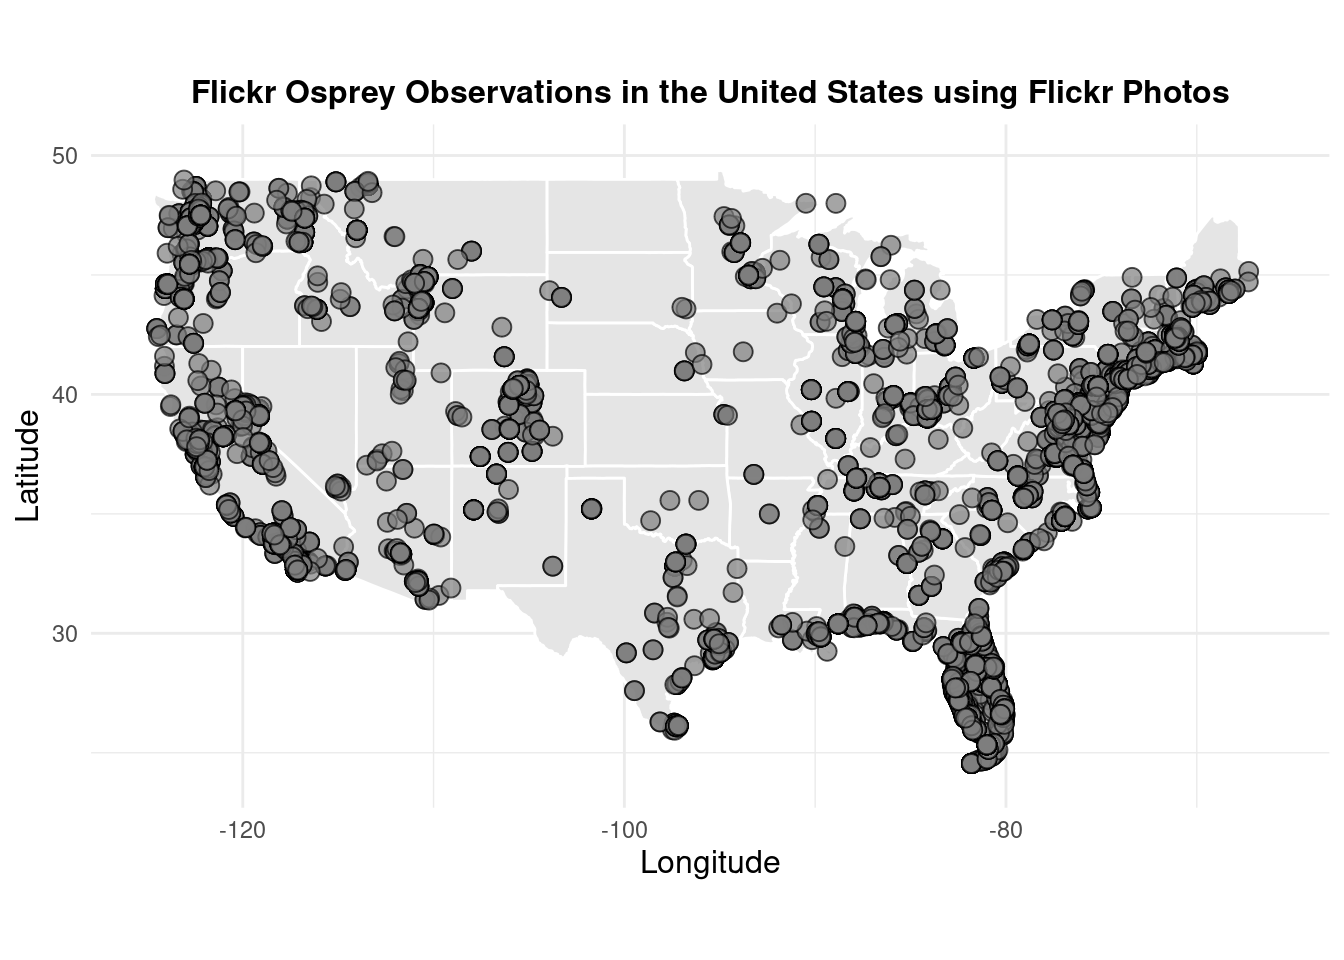
\includegraphics{index_files/figure-pdf/unnamed-chunk-9-1.pdf}

\subsection{Visualizing Seasonal Geodistribution of Ospreys'
Occurrences}\label{visualizing-seasonal-geodistribution-of-ospreys-occurrences}

\begin{Shaded}
\begin{Highlighting}[]
\CommentTok{\#Check the frequency of seasons }
\NormalTok{summer\_frequency }\OtherTok{\textless{}{-}}\NormalTok{ Osprey }\SpecialCharTok{\%\textgreater{}\%}
  \FunctionTok{filter}\NormalTok{(season }\SpecialCharTok{==} \StringTok{"Summer"}\NormalTok{) }\SpecialCharTok{\%\textgreater{}\%}
  \FunctionTok{count}\NormalTok{(state, }\AttributeTok{name =} \StringTok{"frequency"}\NormalTok{) }\SpecialCharTok{\%\textgreater{}\%}
\FunctionTok{arrange}\NormalTok{(}\FunctionTok{desc}\NormalTok{(frequency))}

\NormalTok{winter\_frequency }\OtherTok{\textless{}{-}}\NormalTok{ Osprey }\SpecialCharTok{\%\textgreater{}\%}
  \FunctionTok{filter}\NormalTok{(season }\SpecialCharTok{==} \StringTok{"Winter"}\NormalTok{) }\SpecialCharTok{\%\textgreater{}\%}
  \FunctionTok{count}\NormalTok{(state, }\AttributeTok{name =} \StringTok{"frequency"}\NormalTok{) }\SpecialCharTok{\%\textgreater{}\%}
  \FunctionTok{arrange}\NormalTok{(}\FunctionTok{desc}\NormalTok{(frequency))}

\CommentTok{\#show them as percentage }
\NormalTok{summer\_sum }\OtherTok{\textless{}{-}} \FunctionTok{sum}\NormalTok{(summer\_frequency}\SpecialCharTok{$}\NormalTok{frequency)}
\NormalTok{winter\_sum }\OtherTok{\textless{}{-}} \FunctionTok{sum}\NormalTok{(winter\_frequency}\SpecialCharTok{$}\NormalTok{frequency)}

\NormalTok{summer\_frequency }\OtherTok{\textless{}{-}} \FunctionTok{transform}\NormalTok{(summer\_frequency, }\AttributeTok{percent =}\NormalTok{ frequency }\SpecialCharTok{/}\NormalTok{ summer\_sum }\SpecialCharTok{*} \DecValTok{100}\NormalTok{)}
\NormalTok{winter\_frequency }\OtherTok{\textless{}{-}} \FunctionTok{transform}\NormalTok{(winter\_frequency, }\AttributeTok{percent =}\NormalTok{ frequency }\SpecialCharTok{/}\NormalTok{ winter\_sum }\SpecialCharTok{*} \DecValTok{100}\NormalTok{)}

\NormalTok{summer\_frequency }\OtherTok{\textless{}{-}} \FunctionTok{head}\NormalTok{(summer\_frequency, }\AttributeTok{n =} \DecValTok{5}\NormalTok{)}
\NormalTok{winter\_frequency }\OtherTok{\textless{}{-}} \FunctionTok{head}\NormalTok{(winter\_frequency, }\AttributeTok{n =} \DecValTok{5}\NormalTok{)}

\NormalTok{summer\_frequency}\SpecialCharTok{$}\NormalTok{season }\OtherTok{\textless{}{-}} \StringTok{"Summer"}
\NormalTok{winter\_frequency}\SpecialCharTok{$}\NormalTok{season }\OtherTok{\textless{}{-}} \StringTok{"Winter"}

\NormalTok{seasonal\_occ }\OtherTok{\textless{}{-}} \FunctionTok{rbind}\NormalTok{(summer\_frequency, winter\_frequency)}

\NormalTok{seasonal\_occ }\OtherTok{\textless{}{-}}\NormalTok{ seasonal\_occ }\SpecialCharTok{\%\textgreater{}\%}
  \FunctionTok{mutate}\NormalTok{(}\AttributeTok{state =} \FunctionTok{fct\_reorder}\NormalTok{(state, }\SpecialCharTok{{-}}\NormalTok{frequency))}

\FunctionTok{ggplot}\NormalTok{(seasonal\_occ, }\FunctionTok{aes}\NormalTok{(}\AttributeTok{x =} \FunctionTok{factor}\NormalTok{(state, }\AttributeTok{levels =} \FunctionTok{rev}\NormalTok{(}\FunctionTok{unique}\NormalTok{(state))), }\AttributeTok{y =}\NormalTok{ frequency, }\AttributeTok{fill =}\NormalTok{ season)) }\SpecialCharTok{+}
  \FunctionTok{geom\_bar}\NormalTok{(}\AttributeTok{stat =} \StringTok{"identity"}\NormalTok{, }\AttributeTok{position =} \FunctionTok{position\_dodge}\NormalTok{(}\AttributeTok{width =} \FloatTok{0.8}\NormalTok{), }\AttributeTok{width =} \FloatTok{0.6}\NormalTok{, }\AttributeTok{color =} \StringTok{"black"}\NormalTok{) }\SpecialCharTok{+} 
  \FunctionTok{geom\_text}\NormalTok{(}\FunctionTok{aes}\NormalTok{(}\AttributeTok{label =} \FunctionTok{paste}\NormalTok{(}\FunctionTok{round}\NormalTok{(percent, }\DecValTok{1}\NormalTok{), }\StringTok{"\%"}\NormalTok{)), }
            \AttributeTok{position =} \FunctionTok{position\_dodge}\NormalTok{(}\AttributeTok{width =} \FloatTok{0.8}\NormalTok{), }
            \AttributeTok{vjust =} \SpecialCharTok{{-}}\FloatTok{2.5}\NormalTok{, }\AttributeTok{size =} \FloatTok{3.5}\NormalTok{, }\AttributeTok{color =} \StringTok{"black"}\NormalTok{, }\AttributeTok{fontface =} \StringTok{"bold"}\NormalTok{) }\SpecialCharTok{+}
  \FunctionTok{labs}\NormalTok{(}
    \AttributeTok{title =} \StringTok{"Osprey Seasonal Occurrences by State"}\NormalTok{,}
    \AttributeTok{x =} \StringTok{"State"}\NormalTok{,}
    \AttributeTok{y =} \StringTok{"Percentage of Total Occurrence"}
\NormalTok{  ) }\SpecialCharTok{+}
  \FunctionTok{scale\_fill\_manual}\NormalTok{(}
    \AttributeTok{values =} \FunctionTok{c}\NormalTok{(}\StringTok{"Winter"} \OtherTok{=} \StringTok{"\#1f78b4"}\NormalTok{, }\StringTok{"Summer"} \OtherTok{=} \StringTok{"\#ff7f00"}\NormalTok{), }
    \AttributeTok{labels =} \FunctionTok{c}\NormalTok{(}\StringTok{"Summer"}\NormalTok{, }\StringTok{"Winter"}\NormalTok{), }
    \AttributeTok{name =} \StringTok{"Season"}
\NormalTok{  ) }\SpecialCharTok{+}
  \FunctionTok{theme\_minimal}\NormalTok{() }\SpecialCharTok{+}
  \FunctionTok{theme}\NormalTok{(}
    \AttributeTok{legend.position =} \StringTok{"top"}\NormalTok{,}
    \AttributeTok{plot.title =} \FunctionTok{element\_text}\NormalTok{(}\AttributeTok{size =} \DecValTok{16}\NormalTok{, }\AttributeTok{face =} \StringTok{"bold"}\NormalTok{, }\AttributeTok{hjust =} \FloatTok{0.5}\NormalTok{), }
    \AttributeTok{axis.title.x =} \FunctionTok{element\_text}\NormalTok{(}\AttributeTok{size =} \DecValTok{14}\NormalTok{, }\AttributeTok{face =} \StringTok{"bold"}\NormalTok{),}
    \AttributeTok{axis.title.y =} \FunctionTok{element\_text}\NormalTok{(}\AttributeTok{size =} \DecValTok{14}\NormalTok{, }\AttributeTok{face =} \StringTok{"bold"}\NormalTok{),}
    \AttributeTok{axis.text.x =} \FunctionTok{element\_text}\NormalTok{(}\AttributeTok{size =} \DecValTok{12}\NormalTok{, }\AttributeTok{face =} \StringTok{"bold"}\NormalTok{, }\AttributeTok{angle =} \DecValTok{45}\NormalTok{, }\AttributeTok{hjust =} \DecValTok{1}\NormalTok{), }
    \AttributeTok{axis.text.y =} \FunctionTok{element\_text}\NormalTok{(}\AttributeTok{size =} \DecValTok{12}\NormalTok{, }\AttributeTok{face =} \StringTok{"bold"}\NormalTok{),}
    \AttributeTok{legend.title =} \FunctionTok{element\_text}\NormalTok{(}\AttributeTok{size =} \DecValTok{12}\NormalTok{, }\AttributeTok{face =} \StringTok{"bold"}\NormalTok{),}
    \AttributeTok{legend.text =} \FunctionTok{element\_text}\NormalTok{(}\AttributeTok{size =} \DecValTok{11}\NormalTok{),}
    \AttributeTok{panel.grid.major.y =} \FunctionTok{element\_line}\NormalTok{(}\AttributeTok{color =} \StringTok{"gray80"}\NormalTok{, }\AttributeTok{linetype =} \StringTok{"dashed"}\NormalTok{), }
    \AttributeTok{panel.grid.major.x =} \FunctionTok{element\_blank}\NormalTok{() }
\NormalTok{  ) }\SpecialCharTok{+}
  \FunctionTok{facet\_wrap}\NormalTok{(}\SpecialCharTok{\textasciitilde{}}\NormalTok{ season, }\AttributeTok{scales =} \StringTok{"free"}\NormalTok{, }\AttributeTok{ncol =} \DecValTok{1}\NormalTok{) }\SpecialCharTok{+}
  \FunctionTok{coord\_flip}\NormalTok{() }
\end{Highlighting}
\end{Shaded}

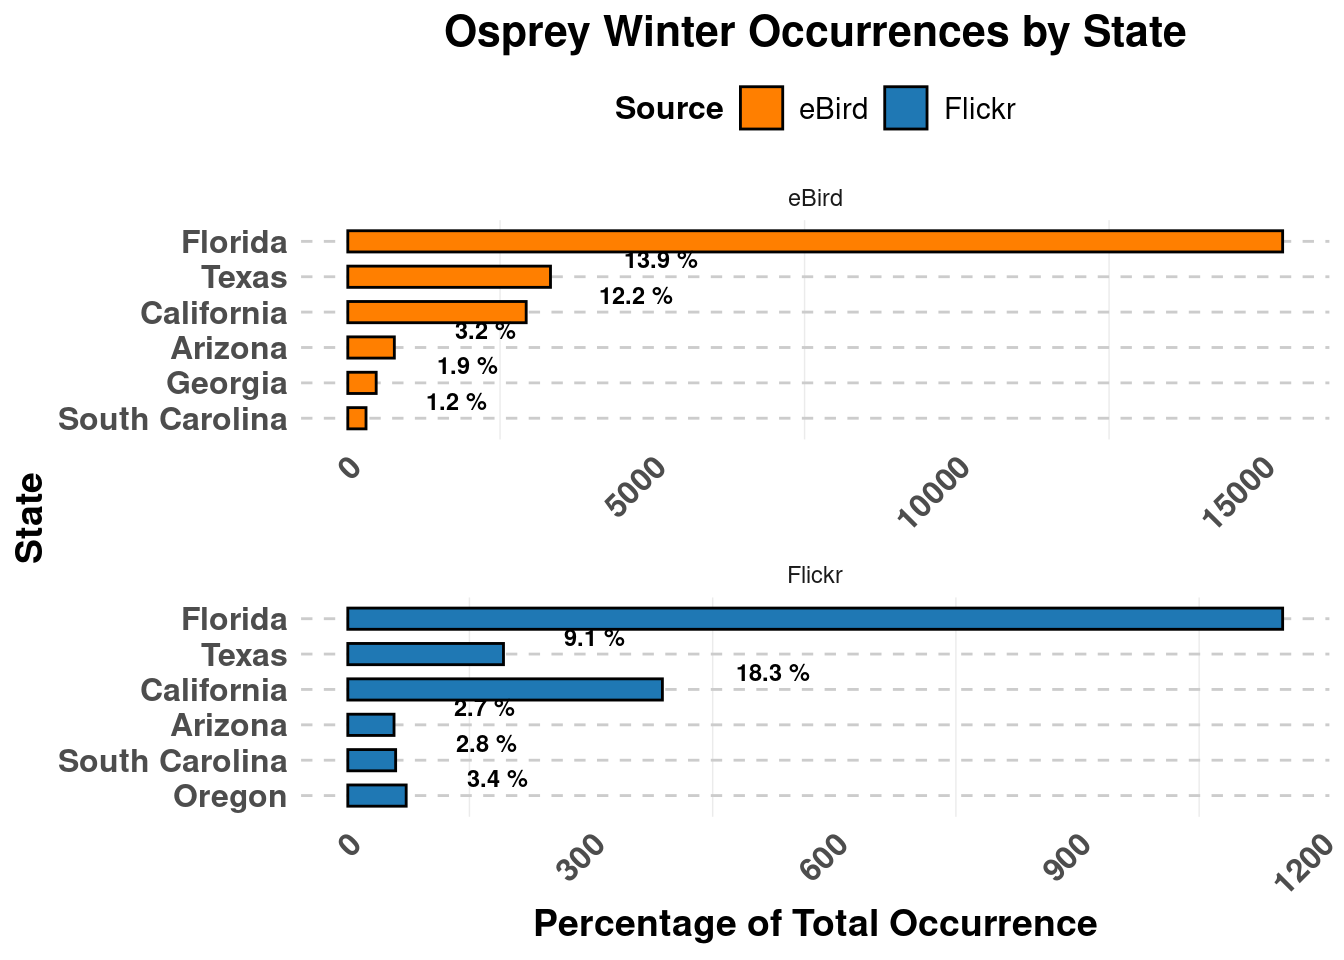
\includegraphics{index_files/figure-pdf/unnamed-chunk-10-1.pdf}

\subsection{Comparing Seasonal Geodistribution of Ospreys from Flickr to
eBird}\label{comparing-seasonal-geodistribution-of-ospreys-from-flickr-to-ebird}

\begin{Shaded}
\begin{Highlighting}[]
\CommentTok{\#Check the frequency of seasons }
\NormalTok{winter\_frequency }\OtherTok{\textless{}{-}}\NormalTok{ Osprey }\SpecialCharTok{\%\textgreater{}\%}
  \FunctionTok{filter}\NormalTok{(season }\SpecialCharTok{==} \StringTok{"Winter"}\NormalTok{) }\SpecialCharTok{\%\textgreater{}\%}
  \FunctionTok{count}\NormalTok{(state, }\AttributeTok{name =} \StringTok{"frequency"}\NormalTok{) }\SpecialCharTok{\%\textgreater{}\%}
  \FunctionTok{arrange}\NormalTok{(}\FunctionTok{desc}\NormalTok{(frequency))}

\NormalTok{winter\_ebird }\OtherTok{\textless{}{-}}\NormalTok{ ebird }\SpecialCharTok{\%\textgreater{}\%}
  \FunctionTok{filter}\NormalTok{(season }\SpecialCharTok{==} \StringTok{"Winter"}\NormalTok{) }\SpecialCharTok{\%\textgreater{}\%}
  \FunctionTok{count}\NormalTok{(STATE, }\AttributeTok{name =} \StringTok{"frequency"}\NormalTok{) }\SpecialCharTok{\%\textgreater{}\%}
  \FunctionTok{arrange}\NormalTok{(}\FunctionTok{desc}\NormalTok{(frequency))}

\NormalTok{winter\_sum }\OtherTok{\textless{}{-}} \FunctionTok{sum}\NormalTok{(winter\_ebird}\SpecialCharTok{$}\NormalTok{frequency)}
\NormalTok{flickr\_win\_sum }\OtherTok{\textless{}{-}} \FunctionTok{sum}\NormalTok{(winter\_frequency}\SpecialCharTok{$}\NormalTok{frequency)}

\NormalTok{winter\_ebird }\OtherTok{\textless{}{-}} \FunctionTok{transform}\NormalTok{(winter\_ebird, }\AttributeTok{percent =}\NormalTok{ frequency }\SpecialCharTok{/}\NormalTok{ winter\_sum }\SpecialCharTok{*} \DecValTok{100}\NormalTok{)}
\NormalTok{winter\_frequency }\OtherTok{\textless{}{-}} \FunctionTok{transform}\NormalTok{(winter\_frequency, }\AttributeTok{percent =}\NormalTok{ frequency }\SpecialCharTok{/}\NormalTok{ flickr\_win\_sum }\SpecialCharTok{*} \DecValTok{100}\NormalTok{)}

\NormalTok{winter\_ebird }\OtherTok{\textless{}{-}} \FunctionTok{head}\NormalTok{(winter\_ebird, }\AttributeTok{n =} \DecValTok{6}\NormalTok{)}
\NormalTok{winter\_frequency }\OtherTok{\textless{}{-}} \FunctionTok{head}\NormalTok{(winter\_frequency, }\AttributeTok{n =} \DecValTok{6}\NormalTok{)}


\NormalTok{winter\_ebird}\SpecialCharTok{$}\NormalTok{source }\OtherTok{\textless{}{-}} \StringTok{"eBird"}
\NormalTok{winter\_frequency}\SpecialCharTok{$}\NormalTok{source }\OtherTok{\textless{}{-}} \StringTok{"Flickr"}

\NormalTok{winter\_ebird }\OtherTok{\textless{}{-}}\NormalTok{ winter\_ebird }\SpecialCharTok{\%\textgreater{}\%}
  \FunctionTok{rename}\NormalTok{(}\AttributeTok{state =}\NormalTok{ STATE) }

\NormalTok{winter\_occ }\OtherTok{\textless{}{-}} \FunctionTok{rbind}\NormalTok{(winter\_ebird, winter\_frequency)}

\NormalTok{winter\_occ }\OtherTok{\textless{}{-}}\NormalTok{ winter\_occ }\SpecialCharTok{\%\textgreater{}\%}
  \FunctionTok{mutate}\NormalTok{(}\AttributeTok{state =} \FunctionTok{fct\_reorder}\NormalTok{(state, }\SpecialCharTok{{-}}\NormalTok{percent))}

\FunctionTok{ggplot}\NormalTok{(winter\_occ, }\FunctionTok{aes}\NormalTok{(}\AttributeTok{x =} \FunctionTok{factor}\NormalTok{(state, }\AttributeTok{levels =} \FunctionTok{rev}\NormalTok{(}\FunctionTok{unique}\NormalTok{(state))), }\AttributeTok{y =}\NormalTok{ frequency, }\AttributeTok{fill =}\NormalTok{ source)) }\SpecialCharTok{+}
  \FunctionTok{geom\_bar}\NormalTok{(}\AttributeTok{stat =} \StringTok{"identity"}\NormalTok{, }\AttributeTok{position =} \FunctionTok{position\_dodge}\NormalTok{(}\AttributeTok{width =} \FloatTok{0.8}\NormalTok{), }\AttributeTok{width =} \FloatTok{0.6}\NormalTok{, }\AttributeTok{color =} \StringTok{"black"}\NormalTok{) }\SpecialCharTok{+} \CommentTok{\# Add border for bars}
  \FunctionTok{geom\_text}\NormalTok{(}\FunctionTok{aes}\NormalTok{(}\AttributeTok{label =} \FunctionTok{paste}\NormalTok{(}\FunctionTok{round}\NormalTok{(percent, }\DecValTok{1}\NormalTok{), }\StringTok{"\%"}\NormalTok{)), }
            \AttributeTok{position =} \FunctionTok{position\_dodge}\NormalTok{(}\AttributeTok{width =} \FloatTok{0.8}\NormalTok{), }
            \AttributeTok{vjust =} \SpecialCharTok{{-}}\FloatTok{0.5}\NormalTok{, }\AttributeTok{hjust =} \SpecialCharTok{{-}}\FloatTok{0.99}\NormalTok{, }\AttributeTok{size =} \FloatTok{3.1}\NormalTok{, }\AttributeTok{color =} \StringTok{"black"}\NormalTok{, }\AttributeTok{fontface =} \StringTok{"bold"}\NormalTok{) }\SpecialCharTok{+}
  \FunctionTok{labs}\NormalTok{(}
    \AttributeTok{title =} \StringTok{"Osprey Winter Occurrences by State"}\NormalTok{,}
    \AttributeTok{x =} \StringTok{"State"}\NormalTok{,}
    \AttributeTok{y =} \StringTok{"Percentage of Total Occurrence"}
\NormalTok{  ) }\SpecialCharTok{+}
  \FunctionTok{scale\_fill\_manual}\NormalTok{(}
    \AttributeTok{values =} \FunctionTok{c}\NormalTok{( }\StringTok{"eBird"} \OtherTok{=} \StringTok{"\#ff7f00"}\NormalTok{, }\StringTok{"Flickr"} \OtherTok{=} \StringTok{"\#1f78b4"}\NormalTok{ ), }
    \AttributeTok{labels =} \FunctionTok{c}\NormalTok{(}\StringTok{"eBird"}\NormalTok{, }\StringTok{"Flickr"}\NormalTok{), }
    \AttributeTok{name =} \StringTok{"Source"}
\NormalTok{  ) }\SpecialCharTok{+}
  \FunctionTok{theme\_minimal}\NormalTok{() }\SpecialCharTok{+}
  \FunctionTok{theme}\NormalTok{(}
    \AttributeTok{legend.position =} \StringTok{"top"}\NormalTok{,}
    \AttributeTok{plot.title =} \FunctionTok{element\_text}\NormalTok{(}\AttributeTok{size =} \DecValTok{16}\NormalTok{, }\AttributeTok{face =} \StringTok{"bold"}\NormalTok{, }\AttributeTok{hjust =} \FloatTok{0.5}\NormalTok{), }
    \AttributeTok{axis.title.x =} \FunctionTok{element\_text}\NormalTok{(}\AttributeTok{size =} \DecValTok{14}\NormalTok{, }\AttributeTok{face =} \StringTok{"bold"}\NormalTok{),}
    \AttributeTok{axis.title.y =} \FunctionTok{element\_text}\NormalTok{(}\AttributeTok{size =} \DecValTok{14}\NormalTok{, }\AttributeTok{face =} \StringTok{"bold"}\NormalTok{),}
    \AttributeTok{axis.text.x =} \FunctionTok{element\_text}\NormalTok{(}\AttributeTok{size =} \DecValTok{12}\NormalTok{, }\AttributeTok{face =} \StringTok{"bold"}\NormalTok{, }\AttributeTok{angle =} \DecValTok{45}\NormalTok{, }\AttributeTok{hjust =} \DecValTok{1}\NormalTok{), }
    \AttributeTok{axis.text.y =} \FunctionTok{element\_text}\NormalTok{(}\AttributeTok{size =} \DecValTok{12}\NormalTok{, }\AttributeTok{face =} \StringTok{"bold"}\NormalTok{),}
    \AttributeTok{legend.title =} \FunctionTok{element\_text}\NormalTok{(}\AttributeTok{size =} \DecValTok{12}\NormalTok{, }\AttributeTok{face =} \StringTok{"bold"}\NormalTok{),}
    \AttributeTok{legend.text =} \FunctionTok{element\_text}\NormalTok{(}\AttributeTok{size =} \DecValTok{11}\NormalTok{),}
    \AttributeTok{panel.grid.major.y =} \FunctionTok{element\_line}\NormalTok{(}\AttributeTok{color =} \StringTok{"gray80"}\NormalTok{, }\AttributeTok{linetype =} \StringTok{"dashed"}\NormalTok{), }
    \AttributeTok{panel.grid.major.x =} \FunctionTok{element\_blank}\NormalTok{() }
\NormalTok{  ) }\SpecialCharTok{+}
  \FunctionTok{facet\_wrap}\NormalTok{(}\SpecialCharTok{\textasciitilde{}}\NormalTok{ source, }\AttributeTok{scales =} \StringTok{"free"}\NormalTok{, }\AttributeTok{ncol =} \DecValTok{1}\NormalTok{) }\SpecialCharTok{+}
  \FunctionTok{coord\_flip}\NormalTok{() }
\end{Highlighting}
\end{Shaded}

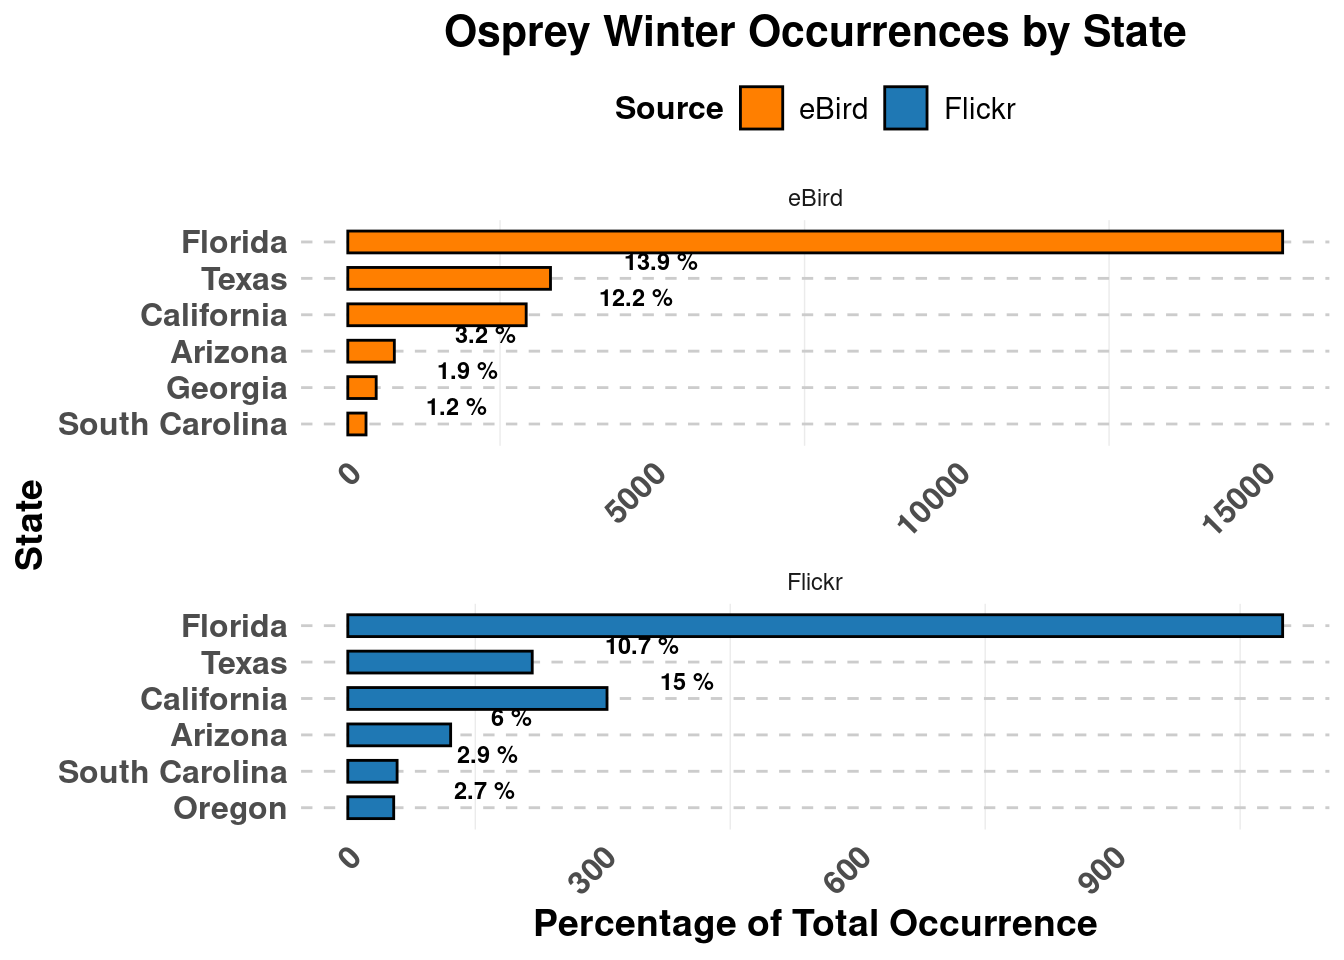
\includegraphics{index_files/figure-pdf/unnamed-chunk-11-1.pdf}

\subsection{Overall Seasonal Trend of
Observations}\label{overall-seasonal-trend-of-observations}

\begin{Shaded}
\begin{Highlighting}[]
\CommentTok{\#Plot of seasons}
\NormalTok{seasons }\OtherTok{\textless{}{-}}\NormalTok{ Osprey }\SpecialCharTok{\%\textgreater{}\%}
  \FunctionTok{group\_by}\NormalTok{(season) }\SpecialCharTok{\%\textgreater{}\%}
  \FunctionTok{summarise}\NormalTok{(}\AttributeTok{Count =} \FunctionTok{n}\NormalTok{()) }\SpecialCharTok{\%\textgreater{}\%}
  \FunctionTok{arrange}\NormalTok{(}\FunctionTok{factor}\NormalTok{(season, }\AttributeTok{levels =} \FunctionTok{c}\NormalTok{(}\StringTok{"Spring"}\NormalTok{, }\StringTok{"Summer"}\NormalTok{, }\StringTok{"Fall"}\NormalTok{, }\StringTok{"Winter"}\NormalTok{)))}

\NormalTok{season\_sum }\OtherTok{\textless{}{-}} \FunctionTok{sum}\NormalTok{(seasons}\SpecialCharTok{$}\NormalTok{Count)}

\NormalTok{seasons }\OtherTok{\textless{}{-}} \FunctionTok{transform}\NormalTok{(seasons, }\AttributeTok{percent =}\NormalTok{ Count }\SpecialCharTok{/}\NormalTok{ season\_sum }\SpecialCharTok{*} \DecValTok{100}\NormalTok{) }\SpecialCharTok{\%\textgreater{}\%}
  \FunctionTok{arrange}\NormalTok{(}\FunctionTok{factor}\NormalTok{(season, }\AttributeTok{levels =} \FunctionTok{c}\NormalTok{(}\StringTok{"Spring"}\NormalTok{, }\StringTok{"Summer"}\NormalTok{, }\StringTok{"Fall"}\NormalTok{, }\StringTok{"Winter"}\NormalTok{)))}

\CommentTok{\#For ebird data}
\NormalTok{seasons\_ebird }\OtherTok{\textless{}{-}}\NormalTok{ ebird }\SpecialCharTok{\%\textgreater{}\%}
  \FunctionTok{group\_by}\NormalTok{(season) }\SpecialCharTok{\%\textgreater{}\%}
  \FunctionTok{summarise}\NormalTok{(}\AttributeTok{Count =} \FunctionTok{n}\NormalTok{()) }\SpecialCharTok{\%\textgreater{}\%}
  \FunctionTok{arrange}\NormalTok{(}\FunctionTok{factor}\NormalTok{(season, }\AttributeTok{levels =} \FunctionTok{c}\NormalTok{(}\StringTok{"Spring"}\NormalTok{, }\StringTok{"Summer"}\NormalTok{, }\StringTok{"Fall"}\NormalTok{, }\StringTok{"Winter"}\NormalTok{)))}

\NormalTok{ebird\_season\_sum }\OtherTok{\textless{}{-}} \FunctionTok{sum}\NormalTok{(seasons\_ebird}\SpecialCharTok{$}\NormalTok{Count)}

\NormalTok{seasons\_ebird }\OtherTok{\textless{}{-}} \FunctionTok{transform}\NormalTok{(seasons\_ebird, }\AttributeTok{percent =}\NormalTok{ Count }\SpecialCharTok{/}\NormalTok{ ebird\_season\_sum }\SpecialCharTok{*} \DecValTok{100}\NormalTok{) }\SpecialCharTok{\%\textgreater{}\%}
  \FunctionTok{arrange}\NormalTok{(}\FunctionTok{factor}\NormalTok{(season, }\AttributeTok{levels =} \FunctionTok{c}\NormalTok{(}\StringTok{"Spring"}\NormalTok{, }\StringTok{"Summer"}\NormalTok{, }\StringTok{"Fall"}\NormalTok{, }\StringTok{"Winter"}\NormalTok{)))}

\NormalTok{seasons\_ebird}\SpecialCharTok{$}\NormalTok{source }\OtherTok{\textless{}{-}} \StringTok{"eBird"}
\NormalTok{seasons}\SpecialCharTok{$}\NormalTok{source }\OtherTok{\textless{}{-}} \StringTok{"Flickr"}

\NormalTok{seasonal\_trend }\OtherTok{\textless{}{-}} \FunctionTok{rbind}\NormalTok{(seasons\_ebird, seasons)}

\FunctionTok{ggplot}\NormalTok{(seasonal\_trend, }\FunctionTok{aes}\NormalTok{(}\AttributeTok{x =} \FunctionTok{factor}\NormalTok{(season, }\AttributeTok{levels =} \FunctionTok{c}\NormalTok{(}\StringTok{"Spring"}\NormalTok{, }\StringTok{"Summer"}\NormalTok{, }\StringTok{"Fall"}\NormalTok{, }\StringTok{"Winter"}\NormalTok{)), }\AttributeTok{y =}\NormalTok{ percent, }\AttributeTok{fill =}\NormalTok{ source)) }\SpecialCharTok{+}
  \FunctionTok{geom\_bar}\NormalTok{(}\AttributeTok{stat =} \StringTok{"identity"}\NormalTok{, }\AttributeTok{position =} \FunctionTok{position\_dodge}\NormalTok{(}\AttributeTok{width =} \FloatTok{0.8}\NormalTok{), }\AttributeTok{width =} \FloatTok{0.7}\NormalTok{) }\SpecialCharTok{+}
  \FunctionTok{geom\_text}\NormalTok{(}\FunctionTok{aes}\NormalTok{(}\AttributeTok{label =} \FunctionTok{paste}\NormalTok{(}\FunctionTok{round}\NormalTok{(percent, }\DecValTok{1}\NormalTok{), }\StringTok{"\%"}\NormalTok{)), }
            \AttributeTok{position =} \FunctionTok{position\_dodge}\NormalTok{(}\AttributeTok{width =} \FloatTok{0.8}\NormalTok{), }
            \AttributeTok{vjust =} \SpecialCharTok{{-}}\FloatTok{0.3}\NormalTok{, }\AttributeTok{size =} \DecValTok{4}\NormalTok{, }\AttributeTok{color =} \StringTok{"black"}\NormalTok{, }\AttributeTok{fontface =} \StringTok{"bold"}\NormalTok{) }\SpecialCharTok{+}
  
  \CommentTok{\# Title and axis labels}
  \FunctionTok{labs}\NormalTok{(}
    \AttributeTok{title =} \StringTok{"Osprey Seasonal Frequency across Data Sources"}\NormalTok{,}
    \AttributeTok{x =} \StringTok{"Season"}\NormalTok{,}
    \AttributeTok{y =} \StringTok{"Percentage of Total Events"}\NormalTok{,}
    \AttributeTok{fill =} \StringTok{"Data Source"}
\NormalTok{  ) }\SpecialCharTok{+}
  \FunctionTok{scale\_fill\_manual}\NormalTok{(}\AttributeTok{values =} \FunctionTok{c}\NormalTok{(}\StringTok{"Flickr"} \OtherTok{=} \StringTok{"\#1f78b4"}\NormalTok{, }\StringTok{"eBird"} \OtherTok{=} \StringTok{"\#ff7f00"}\NormalTok{)) }\SpecialCharTok{+}
  \FunctionTok{theme\_minimal}\NormalTok{(}\AttributeTok{base\_size =} \DecValTok{12}\NormalTok{) }\SpecialCharTok{+}
  \FunctionTok{theme}\NormalTok{(}
    \AttributeTok{plot.title =} \FunctionTok{element\_text}\NormalTok{(}\AttributeTok{size =} \DecValTok{16}\NormalTok{, }\AttributeTok{face =} \StringTok{"bold"}\NormalTok{, }\AttributeTok{hjust =} \FloatTok{0.5}\NormalTok{),}
    \AttributeTok{axis.title.x =} \FunctionTok{element\_text}\NormalTok{(}\AttributeTok{size =} \DecValTok{14}\NormalTok{, }\AttributeTok{face =} \StringTok{"bold"}\NormalTok{, }\AttributeTok{margin =} \FunctionTok{margin}\NormalTok{(}\AttributeTok{t =} \DecValTok{10}\NormalTok{)),}
    \AttributeTok{axis.title.y =} \FunctionTok{element\_text}\NormalTok{(}\AttributeTok{size =} \DecValTok{14}\NormalTok{, }\AttributeTok{face =} \StringTok{"bold"}\NormalTok{, }\AttributeTok{margin =} \FunctionTok{margin}\NormalTok{(}\AttributeTok{r =} \DecValTok{10}\NormalTok{)),}
    \AttributeTok{axis.text.x =} \FunctionTok{element\_text}\NormalTok{(}\AttributeTok{size =} \DecValTok{12}\NormalTok{, }\AttributeTok{angle =} \DecValTok{45}\NormalTok{, }\AttributeTok{hjust =} \DecValTok{1}\NormalTok{, }\AttributeTok{vjust =} \DecValTok{1}\NormalTok{),}
    \AttributeTok{axis.text.y =} \FunctionTok{element\_text}\NormalTok{(}\AttributeTok{size =} \DecValTok{12}\NormalTok{),}
    \AttributeTok{legend.title =} \FunctionTok{element\_text}\NormalTok{(}\AttributeTok{size =} \DecValTok{12}\NormalTok{, }\AttributeTok{face =} \StringTok{"bold"}\NormalTok{),}
    \AttributeTok{legend.text =} \FunctionTok{element\_text}\NormalTok{(}\AttributeTok{size =} \DecValTok{12}\NormalTok{),}
    \AttributeTok{panel.grid.major.y =} \FunctionTok{element\_line}\NormalTok{(}\AttributeTok{color =} \StringTok{"gray80"}\NormalTok{, }\AttributeTok{linetype =} \StringTok{"dashed"}\NormalTok{),}
    \AttributeTok{panel.grid.minor =} \FunctionTok{element\_blank}\NormalTok{(),}
    \AttributeTok{panel.grid.major.x =} \FunctionTok{element\_blank}\NormalTok{()}
\NormalTok{  )}
\end{Highlighting}
\end{Shaded}

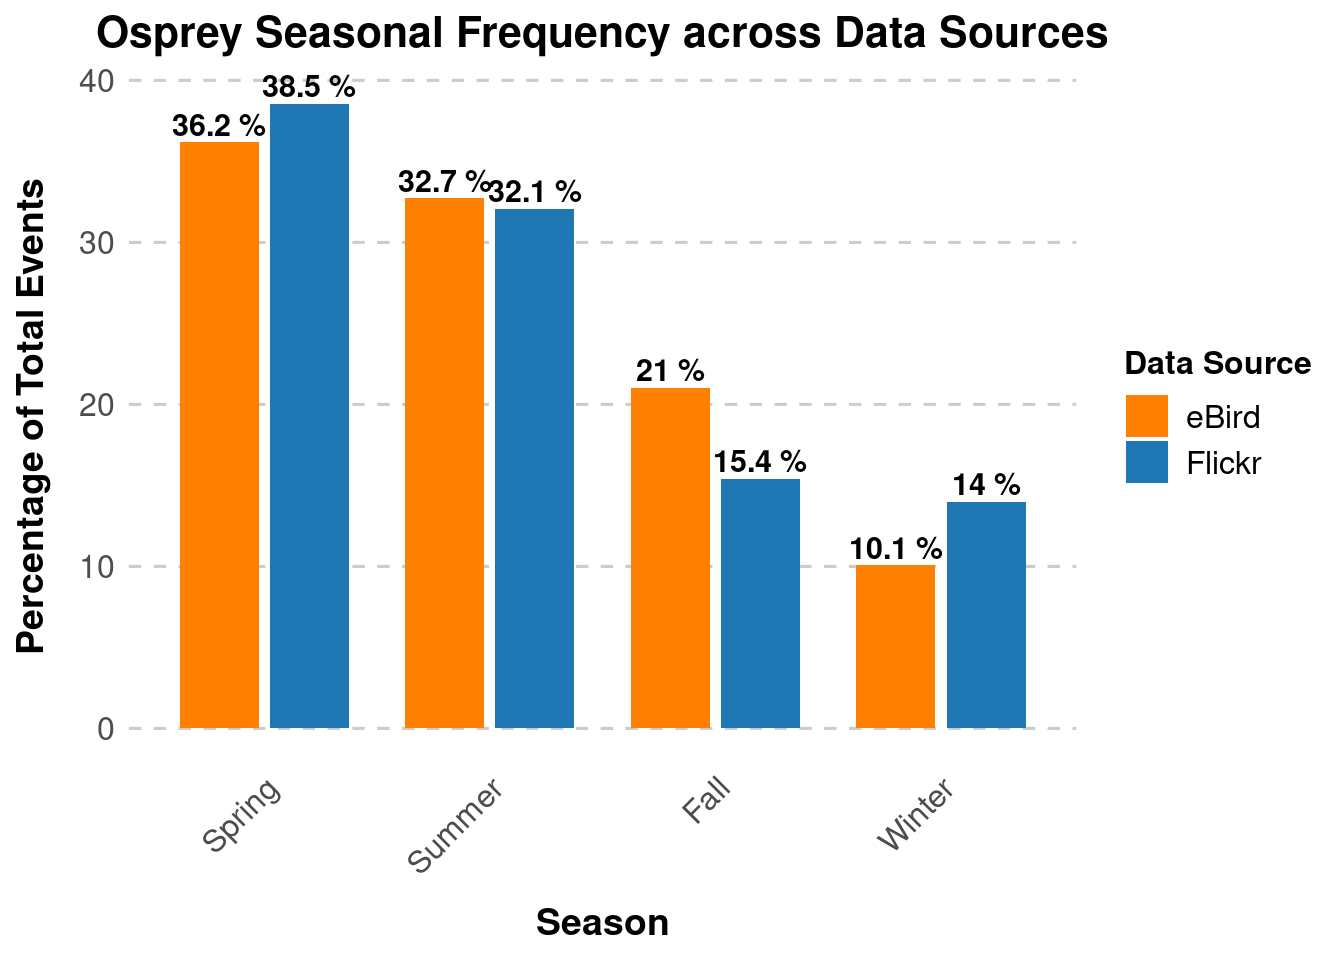
\includegraphics{index_files/figure-pdf/unnamed-chunk-12-1.pdf}

\subsection{Overall GeoDistribution of Ospreys in the US comparing both
datasets}\label{overall-geodistribution-of-ospreys-in-the-us-comparing-both-datasets}

\begin{Shaded}
\begin{Highlighting}[]
\CommentTok{\#State freq}
\NormalTok{State\_frequency }\OtherTok{\textless{}{-}}\NormalTok{ Osprey }\SpecialCharTok{\%\textgreater{}\%}
  \FunctionTok{count}\NormalTok{(state, }\AttributeTok{name =} \StringTok{"frequency"}\NormalTok{) }\SpecialCharTok{\%\textgreater{}\%}
  \FunctionTok{arrange}\NormalTok{(}\FunctionTok{desc}\NormalTok{(frequency))}

\CommentTok{\#State freq}
\NormalTok{State\_ebird }\OtherTok{\textless{}{-}}\NormalTok{ ebird }\SpecialCharTok{\%\textgreater{}\%}
  \FunctionTok{count}\NormalTok{(STATE, }\AttributeTok{name =} \StringTok{"frequency"}\NormalTok{) }\SpecialCharTok{\%\textgreater{}\%}
  \FunctionTok{arrange}\NormalTok{(}\FunctionTok{desc}\NormalTok{(frequency))}

\NormalTok{State\_ebird }\OtherTok{\textless{}{-}} \FunctionTok{head}\NormalTok{(State\_ebird, }\AttributeTok{n =} \DecValTok{10}\NormalTok{)}
\NormalTok{State\_frequency }\OtherTok{\textless{}{-}} \FunctionTok{head}\NormalTok{(State\_frequency, }\AttributeTok{n =} \DecValTok{10}\NormalTok{)}

\NormalTok{ebird\_state\_sum }\OtherTok{\textless{}{-}} \FunctionTok{sum}\NormalTok{(State\_ebird}\SpecialCharTok{$}\NormalTok{frequency)}
\NormalTok{flickr\_season\_sum }\OtherTok{\textless{}{-}} \FunctionTok{sum}\NormalTok{(State\_frequency}\SpecialCharTok{$}\NormalTok{frequency)}

\NormalTok{State\_ebird }\OtherTok{\textless{}{-}} \FunctionTok{transform}\NormalTok{(State\_ebird, }\AttributeTok{percent =}\NormalTok{ frequency}\SpecialCharTok{/}\NormalTok{ ebird\_state\_sum }\SpecialCharTok{*} \DecValTok{100}\NormalTok{) }
\NormalTok{State\_frequency }\OtherTok{\textless{}{-}} \FunctionTok{transform}\NormalTok{(State\_frequency, }\AttributeTok{percent =}\NormalTok{ frequency}\SpecialCharTok{/}\NormalTok{ flickr\_season\_sum }\SpecialCharTok{*} \DecValTok{100}\NormalTok{) }

\NormalTok{State\_ebird}\SpecialCharTok{$}\NormalTok{source }\OtherTok{\textless{}{-}} \StringTok{"eBird"}
\NormalTok{State\_frequency}\SpecialCharTok{$}\NormalTok{source }\OtherTok{\textless{}{-}} \StringTok{"Flickr"}

\NormalTok{State\_ebird }\OtherTok{\textless{}{-}}\NormalTok{ State\_ebird }\SpecialCharTok{\%\textgreater{}\%}
  \FunctionTok{rename}\NormalTok{(}\AttributeTok{state =}\NormalTok{ STATE) }

\NormalTok{state\_trend }\OtherTok{\textless{}{-}} \FunctionTok{rbind}\NormalTok{(State\_ebird, State\_frequency)}

\NormalTok{state\_trend }\OtherTok{\textless{}{-}}\NormalTok{ state\_trend }\SpecialCharTok{\%\textgreater{}\%}
  \FunctionTok{mutate}\NormalTok{(}\AttributeTok{state =} \FunctionTok{fct\_reorder}\NormalTok{(state, }\SpecialCharTok{{-}}\NormalTok{percent))}

\FunctionTok{ggplot}\NormalTok{(state\_trend, }\FunctionTok{aes}\NormalTok{(}\AttributeTok{x =} \FunctionTok{factor}\NormalTok{(state, }\AttributeTok{levels =} \FunctionTok{rev}\NormalTok{(}\FunctionTok{unique}\NormalTok{(state))), }\AttributeTok{y =}\NormalTok{ frequency, }\AttributeTok{fill =}\NormalTok{ source)) }\SpecialCharTok{+}
  \FunctionTok{geom\_bar}\NormalTok{(}\AttributeTok{stat =} \StringTok{"identity"}\NormalTok{, }\AttributeTok{position =} \FunctionTok{position\_dodge}\NormalTok{(}\AttributeTok{width =} \FloatTok{0.8}\NormalTok{), }\AttributeTok{width =} \FloatTok{0.6}\NormalTok{, }\AttributeTok{color =} \StringTok{"black"}\NormalTok{) }\SpecialCharTok{+} 
  \FunctionTok{geom\_text}\NormalTok{(}\FunctionTok{aes}\NormalTok{(}\AttributeTok{label =} \FunctionTok{paste}\NormalTok{(}\FunctionTok{round}\NormalTok{(percent, }\DecValTok{1}\NormalTok{), }\StringTok{"\%"}\NormalTok{)), }
            \AttributeTok{position =} \FunctionTok{position\_dodge}\NormalTok{(}\AttributeTok{width =} \FloatTok{0.8}\NormalTok{), }
            \AttributeTok{vjust =} \SpecialCharTok{{-}}\FloatTok{2.5}\NormalTok{, }\AttributeTok{size =} \FloatTok{3.5}\NormalTok{, }\AttributeTok{color =} \StringTok{"black"}\NormalTok{, }\AttributeTok{fontface =} \StringTok{"bold"}\NormalTok{) }\SpecialCharTok{+}
  \FunctionTok{labs}\NormalTok{(}
    \AttributeTok{title =} \StringTok{"Osprey State Occurrences across Data Source"}\NormalTok{,}
    \AttributeTok{x =} \StringTok{"State"}\NormalTok{,}
    \AttributeTok{y =} \StringTok{"Percentage of Total Occurrence"}
\NormalTok{  ) }\SpecialCharTok{+}
  \FunctionTok{scale\_fill\_manual}\NormalTok{(}
    \AttributeTok{values =} \FunctionTok{c}\NormalTok{( }\StringTok{"eBird"} \OtherTok{=} \StringTok{"\#ff7f00"}\NormalTok{, }\StringTok{"Flickr"} \OtherTok{=} \StringTok{"\#1f78b4"}\NormalTok{ ), }
    \AttributeTok{labels =} \FunctionTok{c}\NormalTok{(}\StringTok{"eBird"}\NormalTok{, }\StringTok{"Flickr"}\NormalTok{), }
    \AttributeTok{name =} \StringTok{"Source"}
\NormalTok{  ) }\SpecialCharTok{+}
  \FunctionTok{theme\_minimal}\NormalTok{() }\SpecialCharTok{+}
  \FunctionTok{theme}\NormalTok{(}
    \AttributeTok{legend.position =} \StringTok{"top"}\NormalTok{,}
    \AttributeTok{plot.title =} \FunctionTok{element\_text}\NormalTok{(}\AttributeTok{size =} \DecValTok{16}\NormalTok{, }\AttributeTok{face =} \StringTok{"bold"}\NormalTok{, }\AttributeTok{hjust =} \FloatTok{0.5}\NormalTok{), }
    \AttributeTok{axis.title.x =} \FunctionTok{element\_text}\NormalTok{(}\AttributeTok{size =} \DecValTok{14}\NormalTok{, }\AttributeTok{face =} \StringTok{"bold"}\NormalTok{),}
    \AttributeTok{axis.title.y =} \FunctionTok{element\_text}\NormalTok{(}\AttributeTok{size =} \DecValTok{14}\NormalTok{, }\AttributeTok{face =} \StringTok{"bold"}\NormalTok{),}
    \AttributeTok{axis.text.x =} \FunctionTok{element\_text}\NormalTok{(}\AttributeTok{size =} \DecValTok{12}\NormalTok{, }\AttributeTok{face =} \StringTok{"bold"}\NormalTok{, }\AttributeTok{angle =} \DecValTok{45}\NormalTok{, }\AttributeTok{hjust =} \DecValTok{1}\NormalTok{), }
    \AttributeTok{axis.text.y =} \FunctionTok{element\_text}\NormalTok{(}\AttributeTok{size =} \DecValTok{12}\NormalTok{, }\AttributeTok{face =} \StringTok{"bold"}\NormalTok{),}
    \AttributeTok{legend.title =} \FunctionTok{element\_text}\NormalTok{(}\AttributeTok{size =} \DecValTok{12}\NormalTok{, }\AttributeTok{face =} \StringTok{"bold"}\NormalTok{),}
    \AttributeTok{legend.text =} \FunctionTok{element\_text}\NormalTok{(}\AttributeTok{size =} \DecValTok{11}\NormalTok{),}
    \AttributeTok{panel.grid.major.y =} \FunctionTok{element\_line}\NormalTok{(}\AttributeTok{color =} \StringTok{"gray80"}\NormalTok{, }\AttributeTok{linetype =} \StringTok{"dashed"}\NormalTok{), }
    \AttributeTok{panel.grid.major.x =} \FunctionTok{element\_blank}\NormalTok{() }
\NormalTok{  ) }\SpecialCharTok{+}
  \FunctionTok{facet\_wrap}\NormalTok{(}\SpecialCharTok{\textasciitilde{}}\NormalTok{ source, }\AttributeTok{scales =} \StringTok{"free"}\NormalTok{, }\AttributeTok{ncol =} \DecValTok{1}\NormalTok{) }\SpecialCharTok{+}
  \FunctionTok{coord\_flip}\NormalTok{() }
\end{Highlighting}
\end{Shaded}

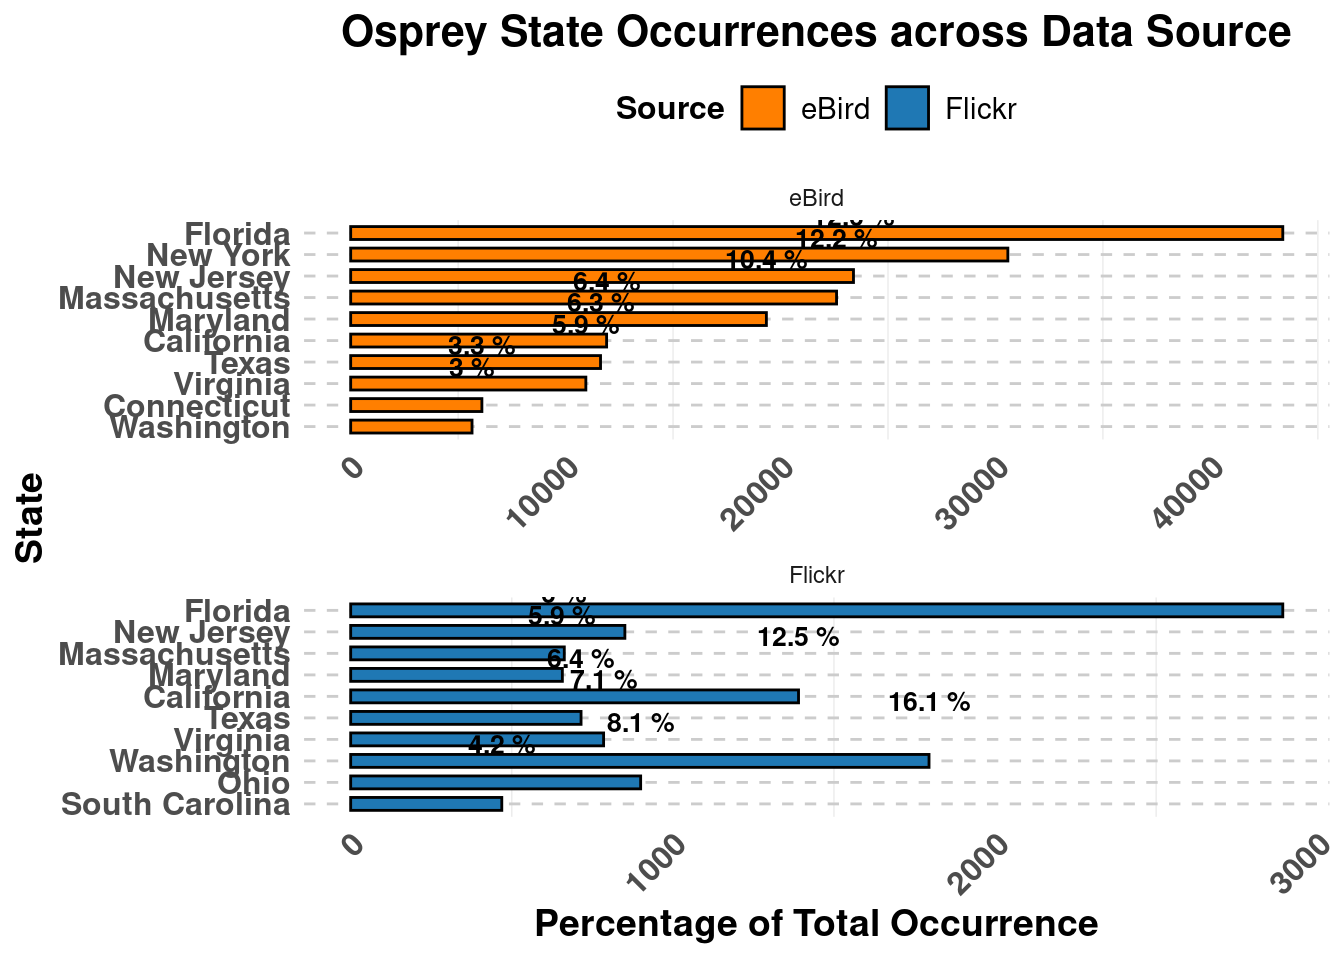
\includegraphics{index_files/figure-pdf/unnamed-chunk-13-1.pdf}

\section{Results}\label{results}

The analysis of Flickr and eBird data reveals consistent trends in the
seasonal distribution of Ospreys across the United States. Flickr photos
indicate clear seasonal migration patterns, with Ospreys predominantly
observed in northern states like New Jersey and Maryland during the
summer months, followed by a shift to southern states such as Florida,
California, Texas, Arizona, and North Carolina during the winter (Figure
2).

A closer examination of the winter distribution shows strong alignment
between the two datasets. The top four states with the highest recorded
Osprey occurrences during winter are identical in both Flickr and eBird
data (Figure 3), highlighting a high level of correlation between the
two sources.

Flickr and eBird data exhibit consistent trends in the seasonal
distribution of Ospreys across the United States, spanning spring,
summer, fall, and winter (Figure 4).Furthermore, when comparing the top
ten states where Ospreys are observed year-round, nine of these states
match between Flickr and eBird datasets (Figure 5).

\section{Conclusions}\label{conclusions}

The high degree of correlation between the two data sources,
particularly in the top states for winter occurrences and year-round
presence, highlights the reliability of photo-based citizen science data
in reflecting species distribution patterns. These findings underscore
the value of integrating alternative data sources like Flickr with
traditional ecological datasets to enhance spatial and temporal
coverage, offering a scalable approach to support conservation and
monitoring efforts for migratory species like the Osprey.

\section{References}\label{references}

\begin{enumerate}
\def\labelenumi{\arabic{enumi}.}
\item
  Bierregaard, R. O., Poole, A. F., \& Washburn, B. E. (2014). Ospreys
  (Pandion haliaetus) in the 21st century: populations, migration,
  management, and research priorities. Journal of Raptor Research,
  48(4), 301-308.
\item
  Martell, M. S., Bierregaard Jr, R. O., Washburn, B. E., Elliott, J.
  E., Henny, C. J., Kennedy, R. S., \& MacLeod, I. (2014). The spring
  migration of adult North American Ospreys. Journal of Raptor Research,
  48(4), 309-324.
\item
  Martell, M. S., Henny, C. J., Nye, P. E., \& Solensky, M. J. (2001).
  Fall migration routes, timing, and wintering sites of North American
  Ospreys as determined by satellite telemetry. The Condor, 103(4),
  715-724.
\item
  Monti, F., Grémillet, D., Sforzi, A., Sammuri, G., Dominici, J. M.,
  Triay Bagur, R., \ldots{} \& Duriez, O. (2018). Migration and
  wintering strategies in vulnerable Mediterranean Osprey populations.
  Ibis, 160(3), 554-567.
\item
  Henny, C. J., Grove, R. A., Kaiser, J. L., \& Johnson, B. L. (2010).
  North American osprey populations and contaminants: historic and
  contemporary perspectives. Journal of Toxicology and Environmental
  Health, Part B, 13(7-8), 579-603.
\end{enumerate}



\end{document}
